\chapter{Réalisation et présentation du MVP de la plateforme des bénéficiaires}
\markboth{CHAPITRE 5. RÉALISATION DU MVP DE LA PLATEFORME}{CHAPITRE 5. RÉALISATION DU MVP DE LA PLATEFORME}

\section{Introduction}

La formalisation du document de référence {\ttfamily Cahier\allowbreak\_\allowbreak des\allowbreak\_\allowbreak Charges\allowbreak\_\allowbreak FOCP\allowbreak\_\allowbreak V3.pdf} par l'application Secure Requirements Studio (SRS) a permis d'établir avec une grande précision l'ensemble des spécifications fonctionnelles, techniques et de cybersécurité de la future plateforme cible de la Fondation OCP. Afin de concrétiser cette démarche d'ingénierie et d'apporter une preuve de concept opérationnelle, nous avons développé le \textbf{MVP (Minimum Viable Product)} de la \textbf{plateforme de gestion des bénéficiaires de l'Axe Social et Solidaire}.

Ce cinquième chapitre est dédié à la présentation détaillée de ce prototype fonctionnel. Nous y exposons les objectifs et le périmètre retenus pour le MVP, décrivons son architecture fonctionnelle modulaire, détaillons l'ensemble de ses interfaces graphiques réelles, et analysons la matrice de conformité et de traçabilité attestant de la parfaite adéquation entre le Cahier des Charges généré et le démonstrateur réalisé.

\section{Objectifs et périmètre du MVP}

Le MVP a été conçu comme une implémentation de référence hautement représentative des processus métier de l'Axe Social et Solidaire. Il vise les objectifs opérationnels suivants :

\begin{itemize}
    \item \textbf{Démontrer la faisabilité technique} de la centralisation des données pour un réseau national de 1\,700 coopératives réparties sur les douze régions du Royaume.
    \item \textbf{Valider le contrôle d'accès basé sur les rôles (RBAC)} en instanciant les espaces différenciés pour les Administrateurs Fondation OCP et les Représentants de coopératives.
    \item \textbf{Dématérialiser le workflow mensuel de reporting} comprenant la saisie des bénéficiaires (directs et indirects), le calcul des parités, la soumission et les actions de validation ou de rejet motivé.
    \item \textbf{Offrir une visualisation géographique interactive} facilitant le repérage spatial des coopératives et l'analyse territoriale des actions de la Fondation.
    \item \textbf{Piloter les indicateurs d'impact durable} par la consolidation automatisée des métriques ESG et des Objectifs de Développement Durable (ODD).
\end{itemize}

\section{Architecture fonctionnelle du MVP}

L'architecture du MVP s'articule autour de modules interconnectés garantissant la modularité, la sécurité et la fluidité des traitements :

\begin{enumerate}
    \item \textbf{Module d'Authentification et Sécurité RBAC} : Gestion des sessions sécurisées, contrôle strict des privilèges et traçabilité des connexions.
    \item \textbf{Module Tableau de Bord Décisionnel} : Agrégation temps réel des KPI d'impact, distribution par genre et suivi de l'évolution mensuelle.
    \item \textbf{Module Annuaire des Coopératives} : Fiches détaillées, contacts, statut juridique, filière d'activité et gouvernance.
    \item \textbf{Module Cartographie Interactive (SIG)} : Visualisation cartographique dynamique avec regroupement par clusters et filtres multicritères.
    \item \textbf{Module Déclarations \& Rapports Mensuels} : Saisie structurée, calcul automatique des bénéficiaires et circuit de validation avec historique.
    \item \textbf{Module Conventions \& Gestion Budgétaire} : Suivi des engagements contractuels, taux de consommation budgétaire et échéanciers.
    \item \textbf{Module Gestion Électronique des Documents (GED)} : Téléversement sécurisé des pièces justificatives, validation et horodatage.
    \item \textbf{Module Moteur d'Importation \& Exportation} : Traitement par lots via fichiers CSV, et génération de rapports de synthèse (Excel, PDF).
    \item \textbf{Module Centre de Notifications} : Alertes contextuelles sur les échéances de reporting et les retours de validation.
\end{enumerate}

\section{Principales interfaces graphiques du prototype MVP}

Nous présentons ci-après l'ensemble des treize interfaces développées pour le MVP de la plateforme de gestion des bénéficiaires.

\subsection{Accueil et authentification sécurisée (RBAC)}

L'écran d'accueil et d'authentification (figure \ref{fig:mvp_01_auth}) constitue le point d'entrée unique de la plateforme. Il intègre une authentification robuste permettant d'orienter l'utilisateur vers son espace dédié selon son rôle : \textit{Administrateur Fondation} ou \textit{Représentant de Coopérative}.

\begin{figure}[H]
\centering
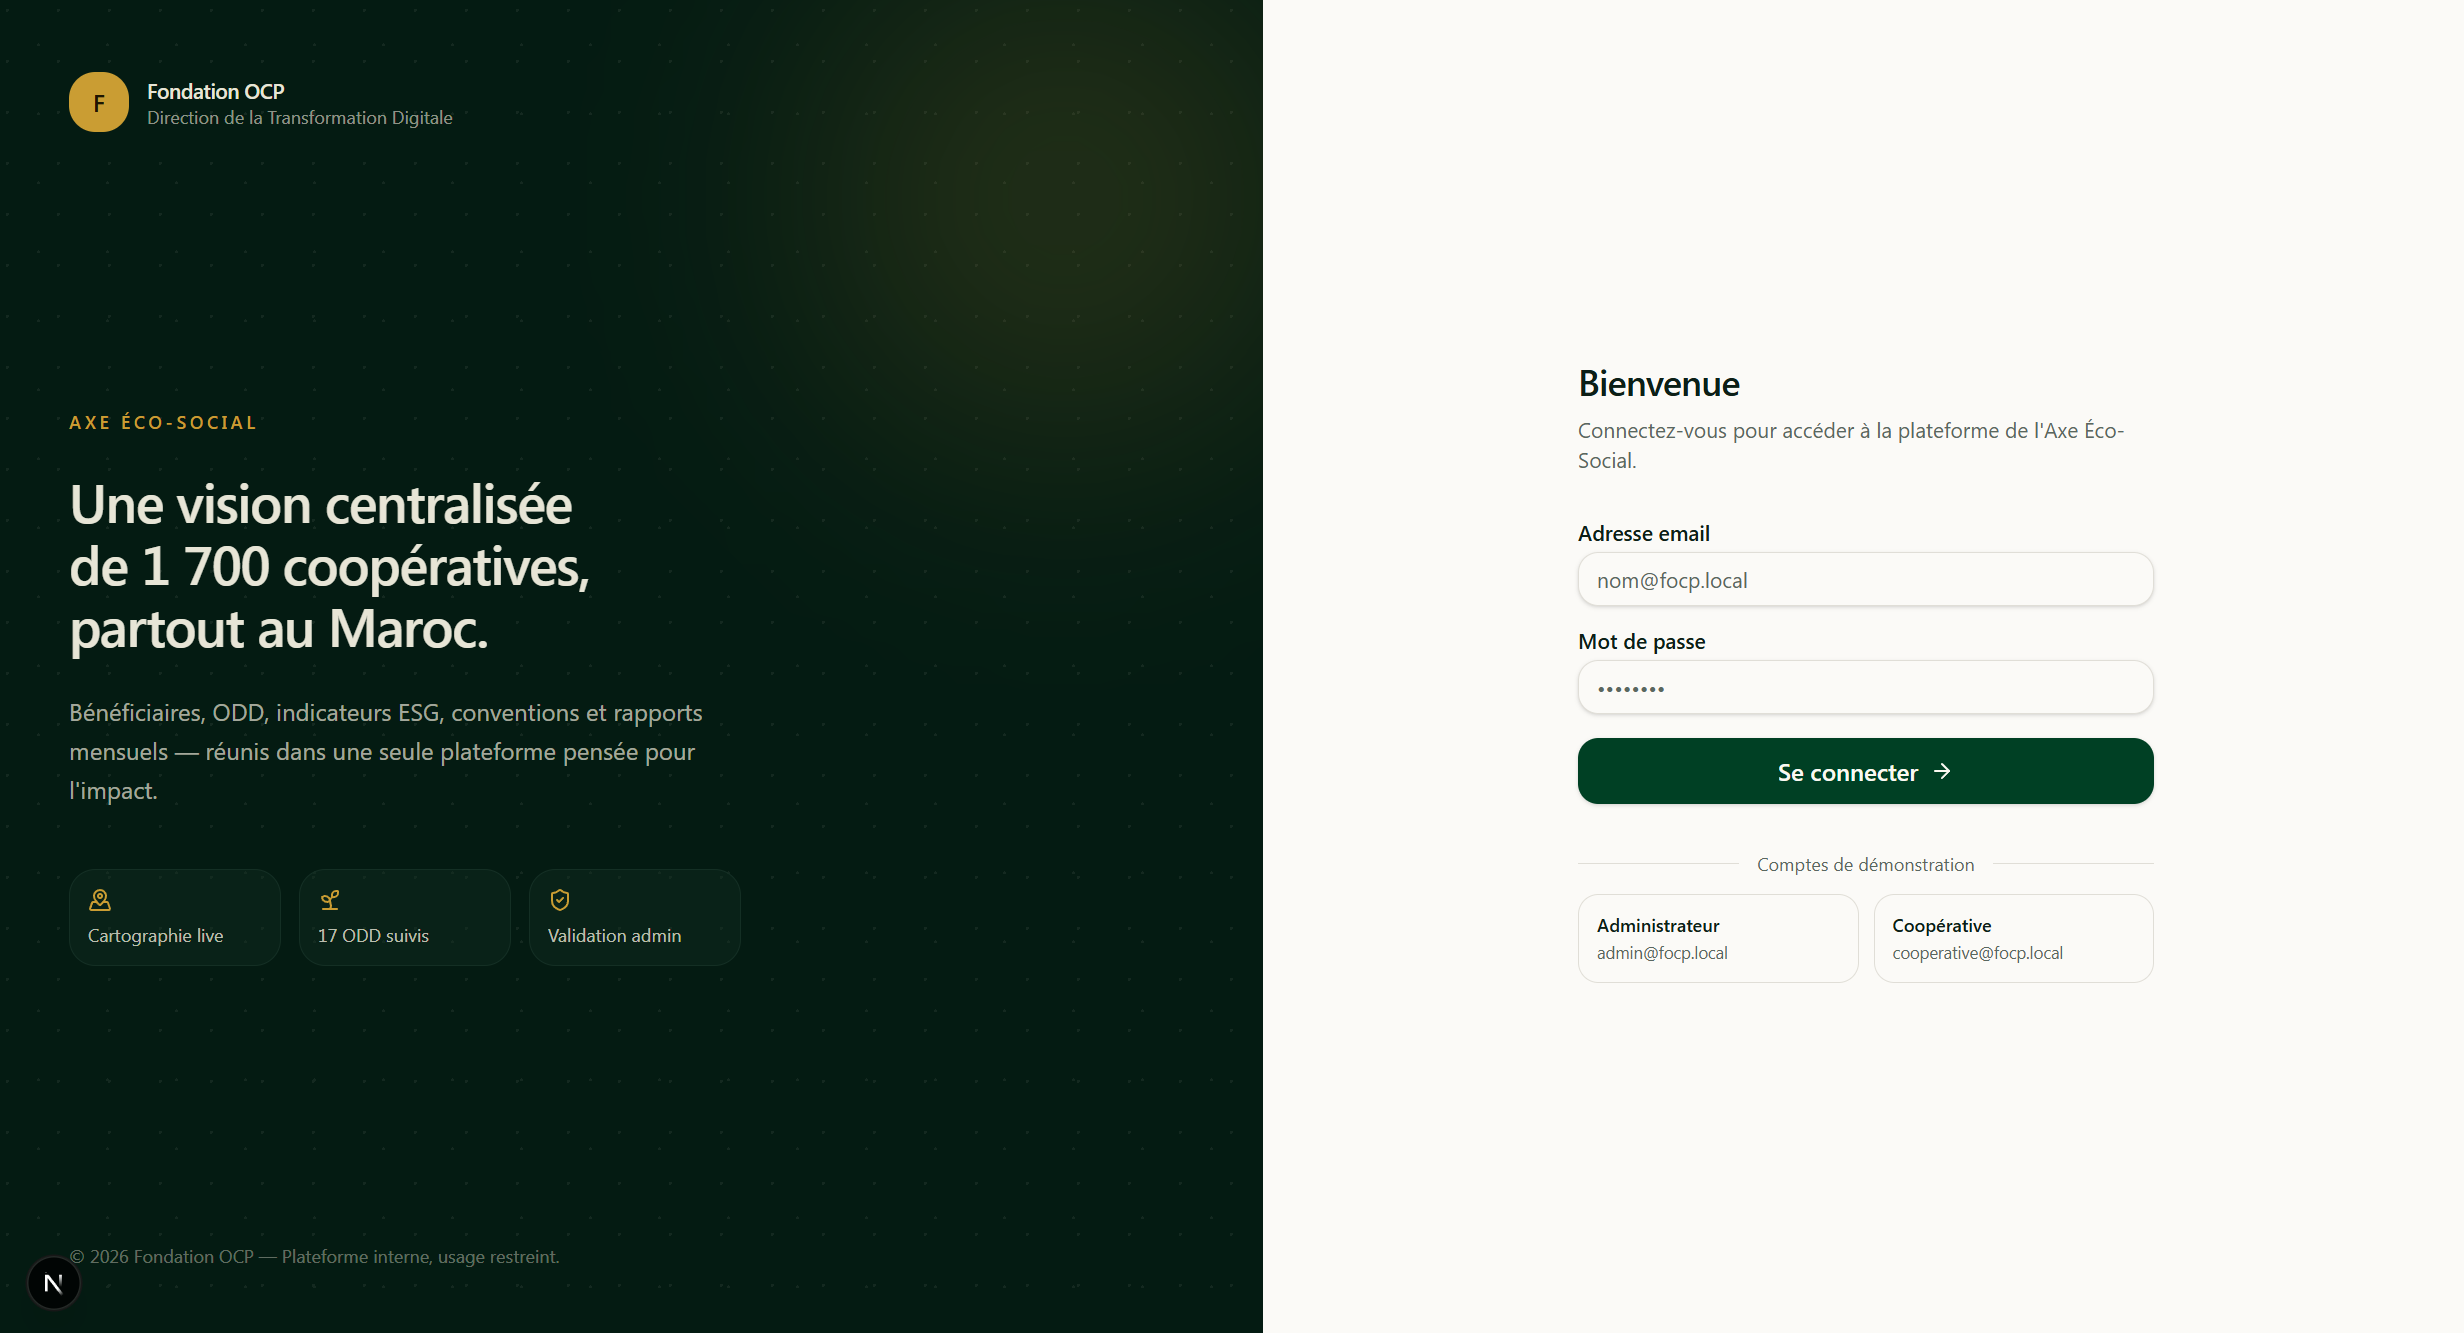
\includegraphics[width=0.90\textwidth]{figures/screenshots/mvp/01_mvp_authentification.png}
\caption{Interface d'accueil et d'authentification sécurisée (RBAC)}
\label{fig:mvp_01_auth}
\end{figure}

Cette interface assure le respect des politiques de sécurité spécifiées (mots de passe forts, protection contre les attaques par force brute et limitation de session).

\subsection{Tableau de bord général de pilotage de l'Axe Social et Solidaire}

Le tableau de bord principal (figure \ref{fig:mvp_02_dash}) offre une vue panoramique et décisionnelle sur l'ensemble du réseau national. Il affiche en temps réel :
\begin{itemize}
    \item Le nombre total de coopératives actives et de conventions signées.
    \item Le volume consolidé des bénéficiaires directs (femmes, jeunes, handicapés, agriculteurs) et indirects.
    \item La répartition des projets selon les Objectifs de Développement Durable (ODD 1, 5, 8, 10, etc.).
    \item L'évolution mensuelle des bénéficiaires et le taux de conformité des rapports déposés.
\end{itemize}

\begin{figure}[H]
\centering
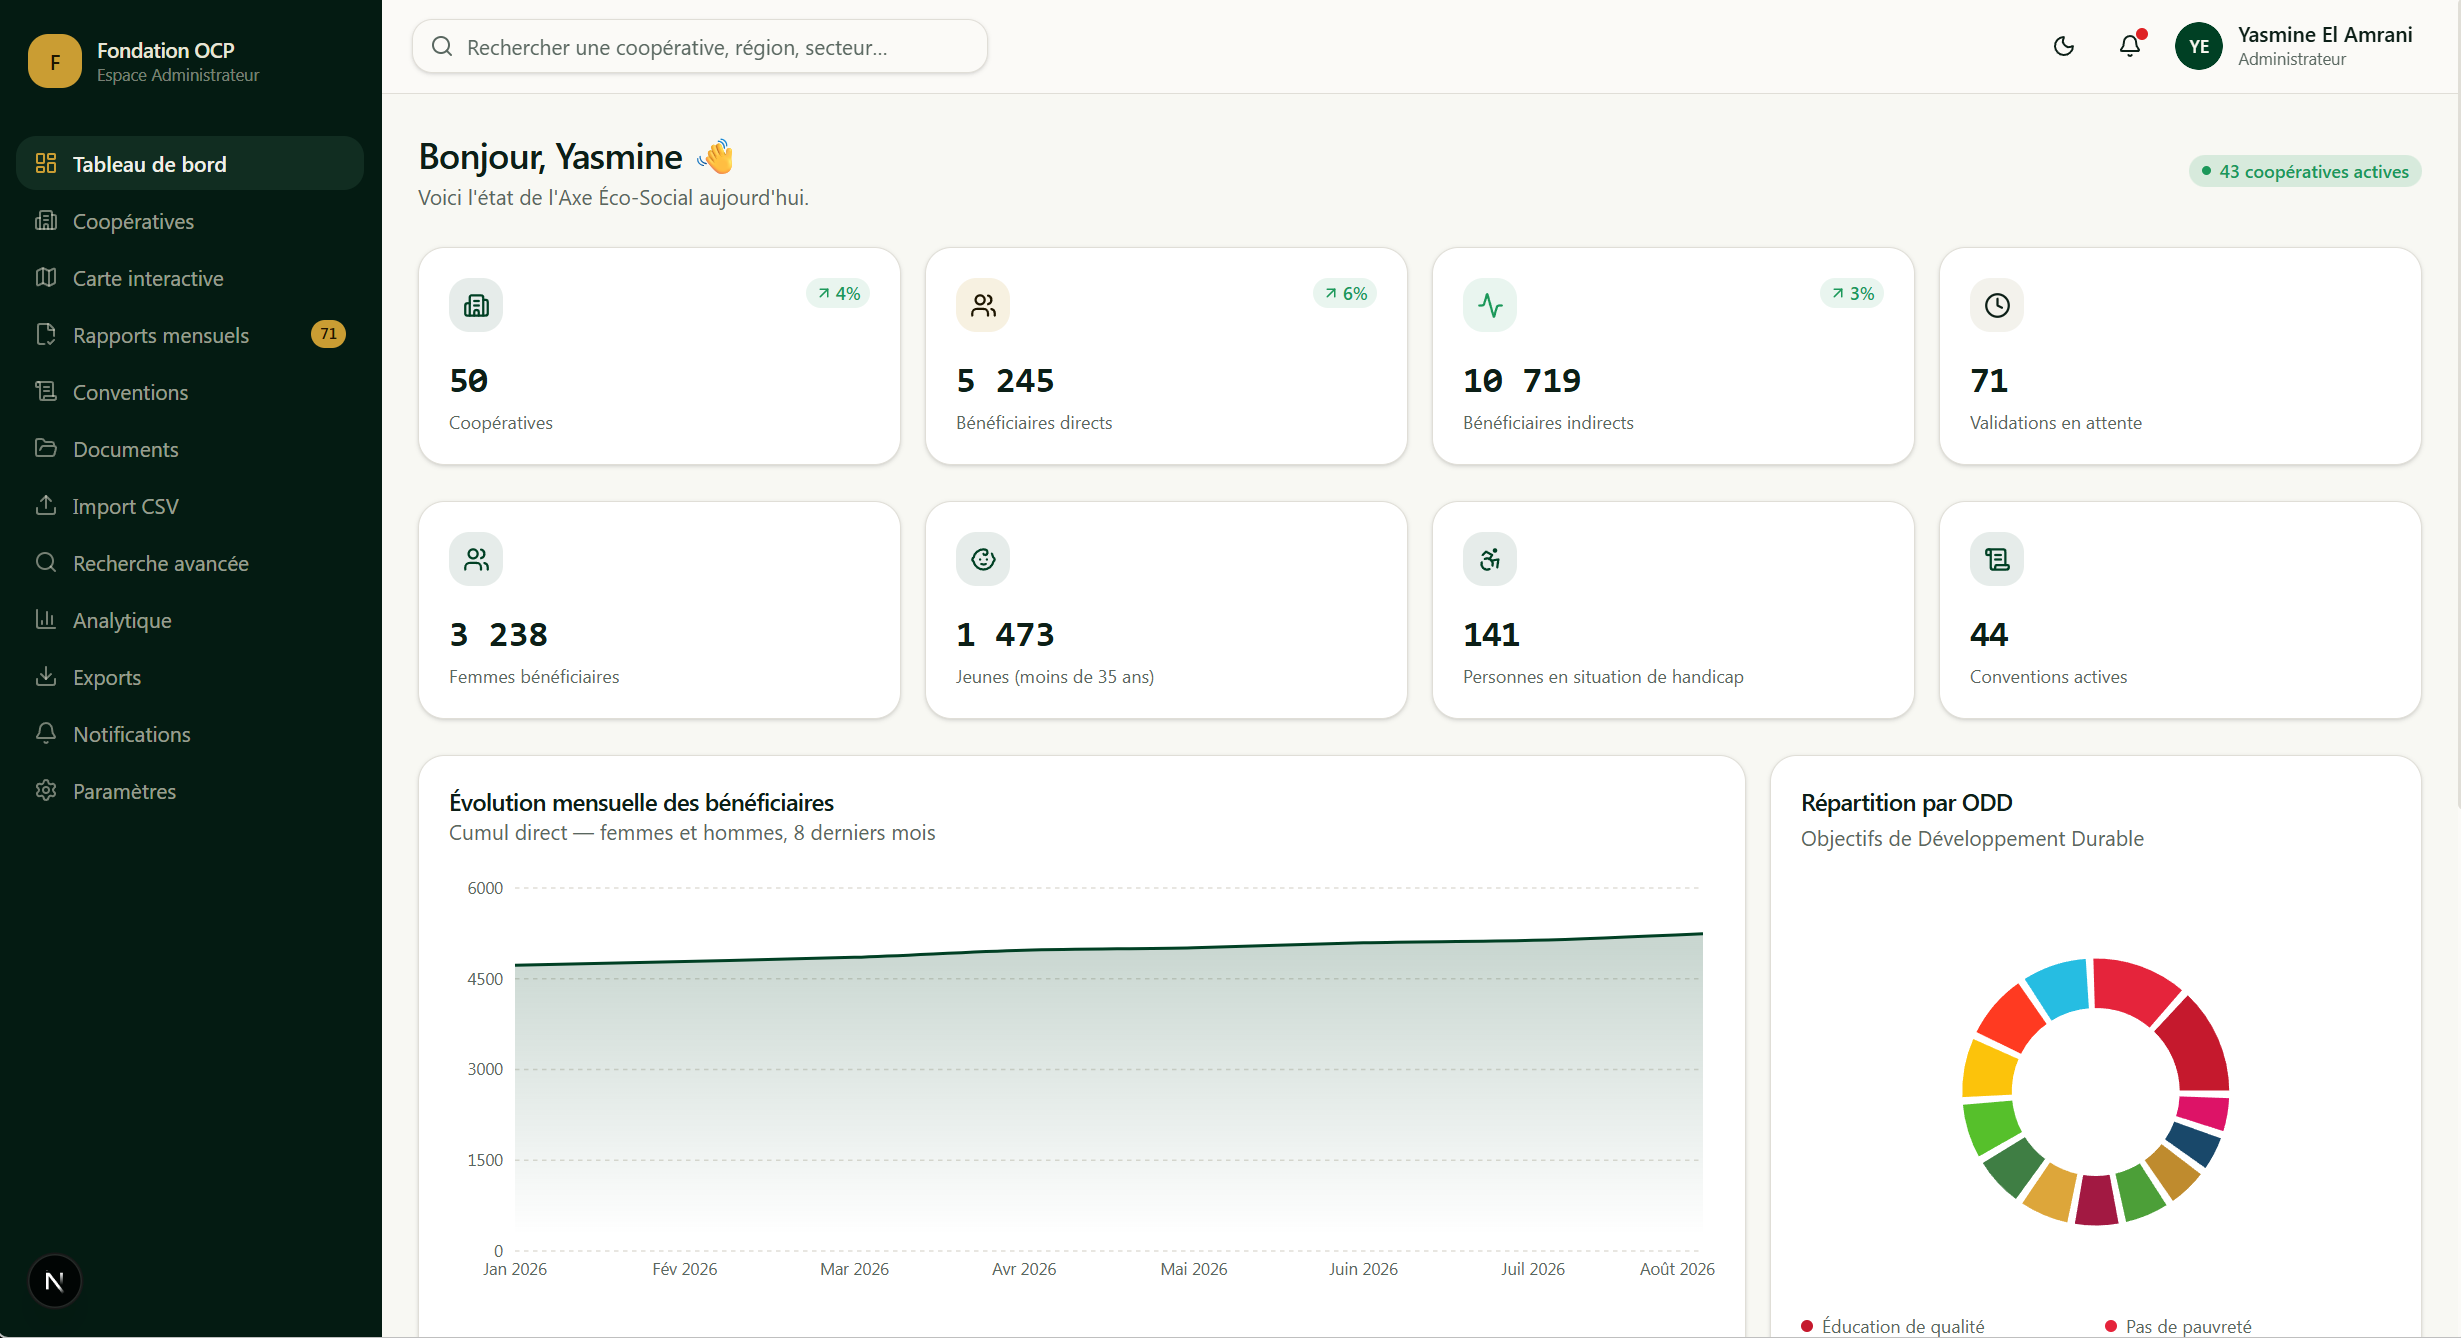
\includegraphics[width=0.90\textwidth]{figures/screenshots/mvp/02_mvp_dashboard.png}
\caption{Tableau de bord général de supervision et indicateurs d'impact}
\label{fig:mvp_02_dash}
\end{figure}

\subsection{Annuaire et gestion des coopératives partenaires}

L'annuaire des coopératives (figure \ref{fig:mvp_03_coop}) permet de gérer l'exhaustivité des 1\,700 coopératives partenaires. L'administrateur peut y filtrer les entités par région, province, secteur d'activité (Artisanat, Agriculture, Argan, Cosmétique, etc.) et statut administratif.

\begin{figure}[H]
\centering
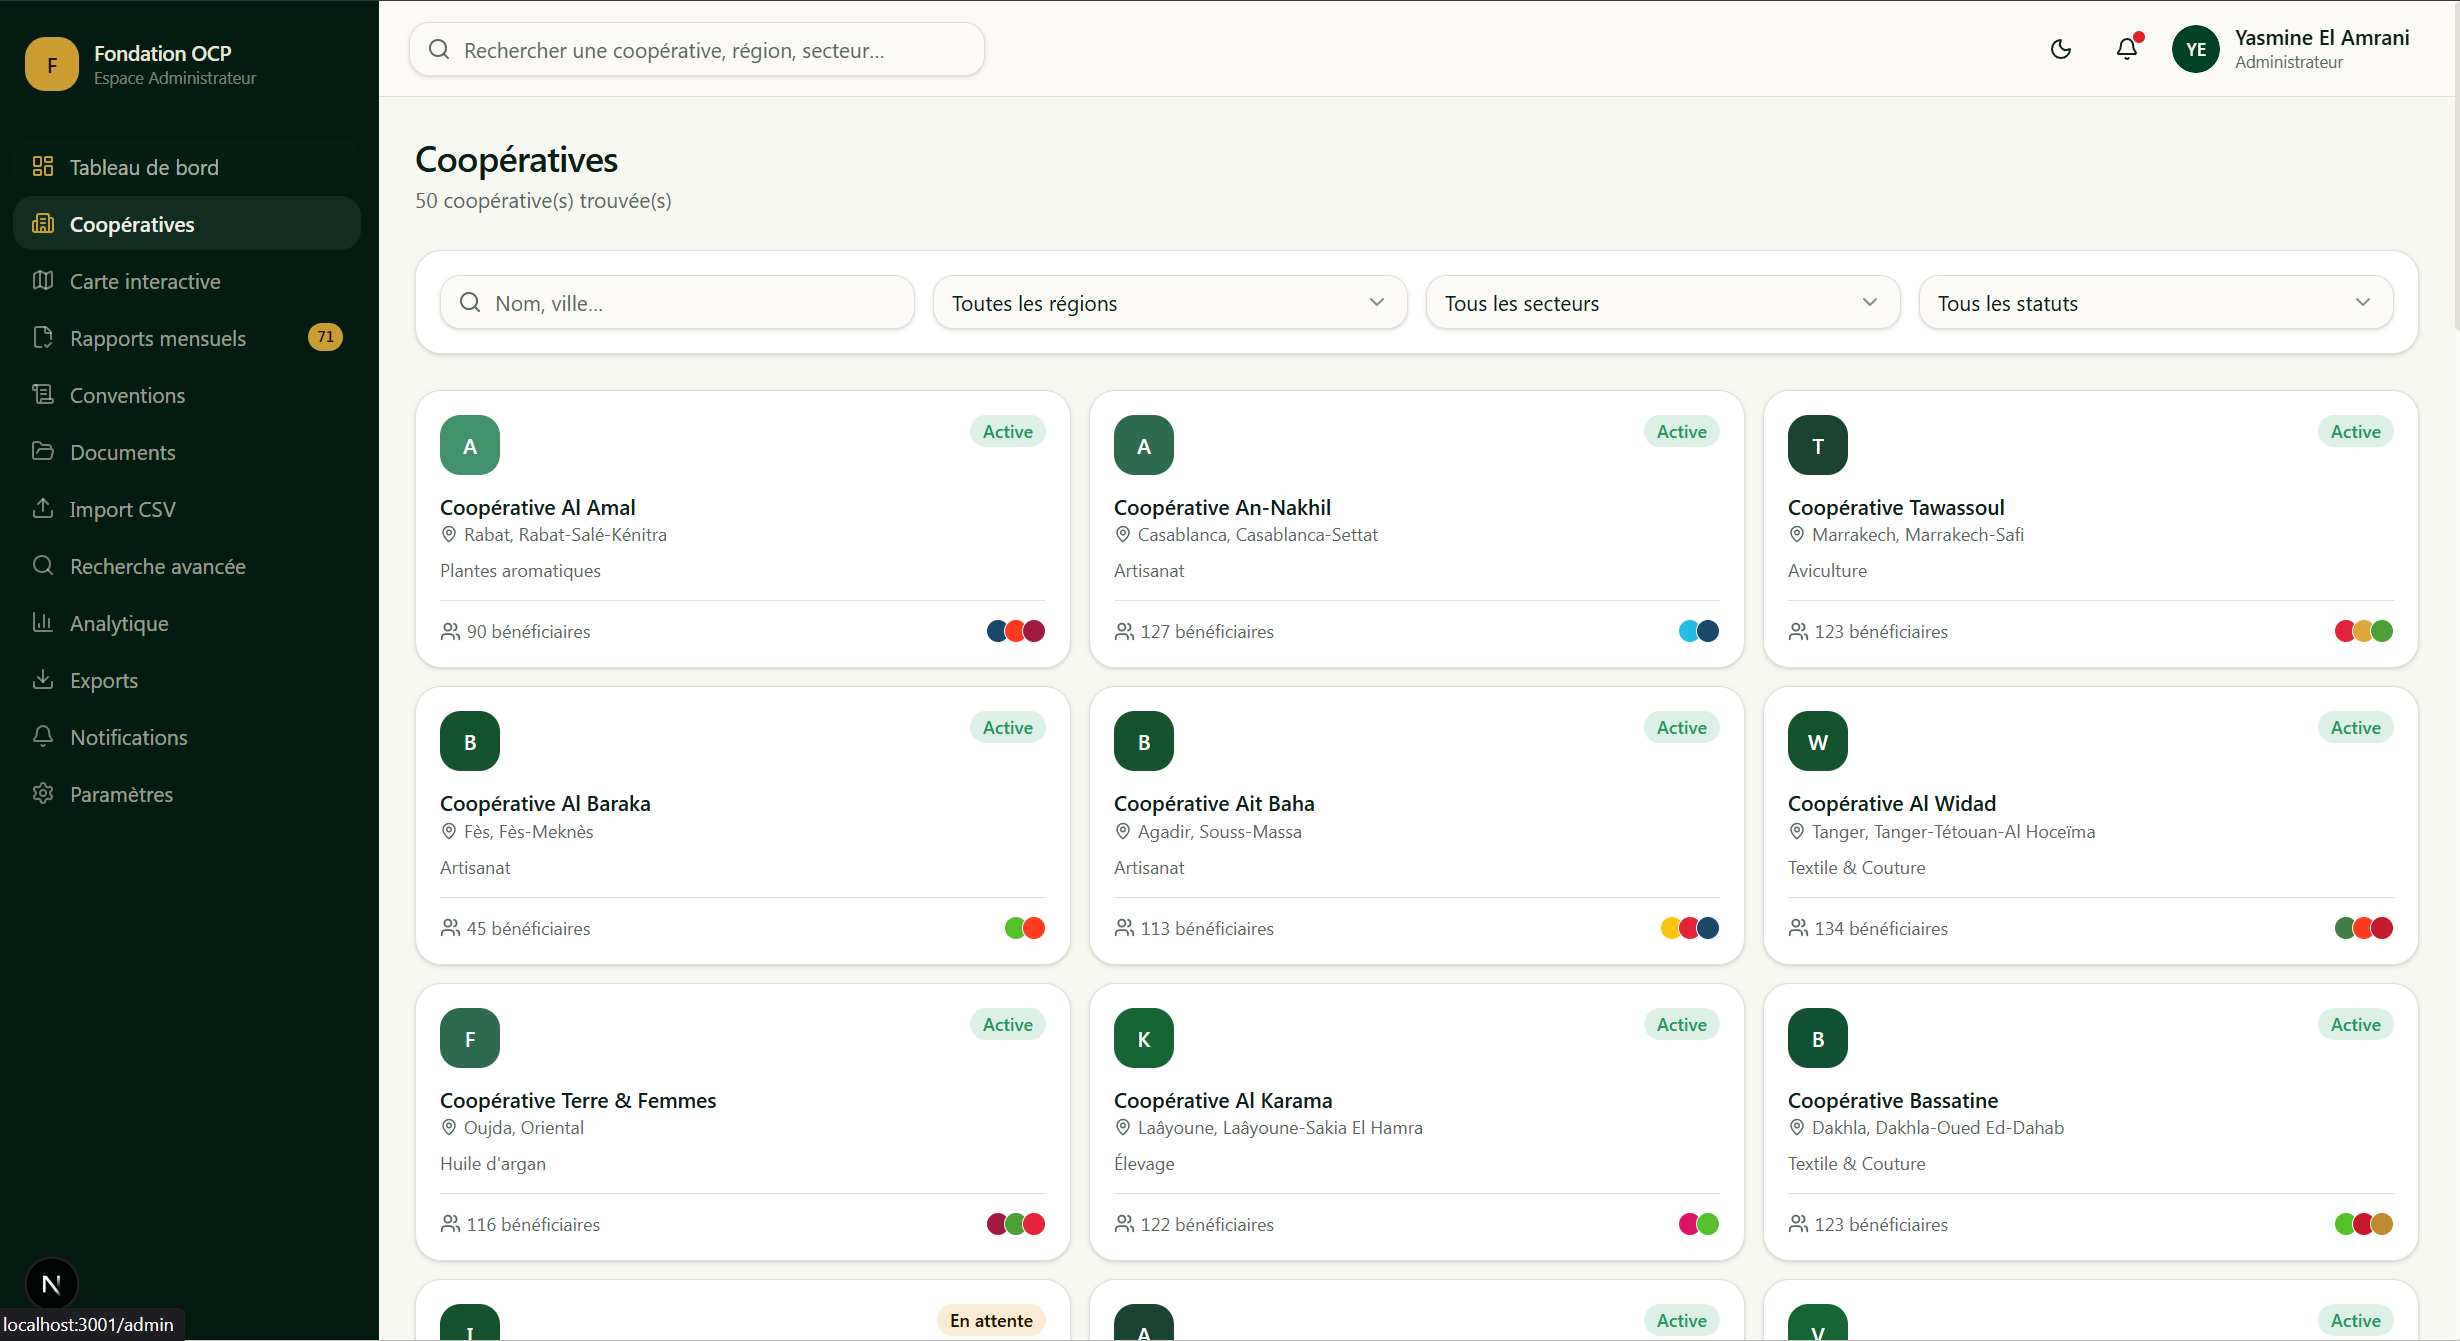
\includegraphics[width=0.90\textwidth]{figures/screenshots/mvp/03_mvp_cooperatives.png}
\caption{Annuaire et gestion détaillée des coopératives partenaires}
\label{fig:mvp_03_coop}
\end{figure}

Chaque ligne permet d'accéder à la fiche individuelle de la coopérative, regroupant ses coordonnées, ses représentants légaux, ses conventions et son historique de déclarations.

\subsection{Cartographie interactive nationale des coopératives}

Le module cartographique (figure \ref{fig:mvp_04_map}) s'appuie sur une carte interactive du Maroc permettant la géolocalisation précise des coopératives et l'analyse territoriale des retombées des programmes de la Fondation OCP.

\begin{figure}[H]
\centering
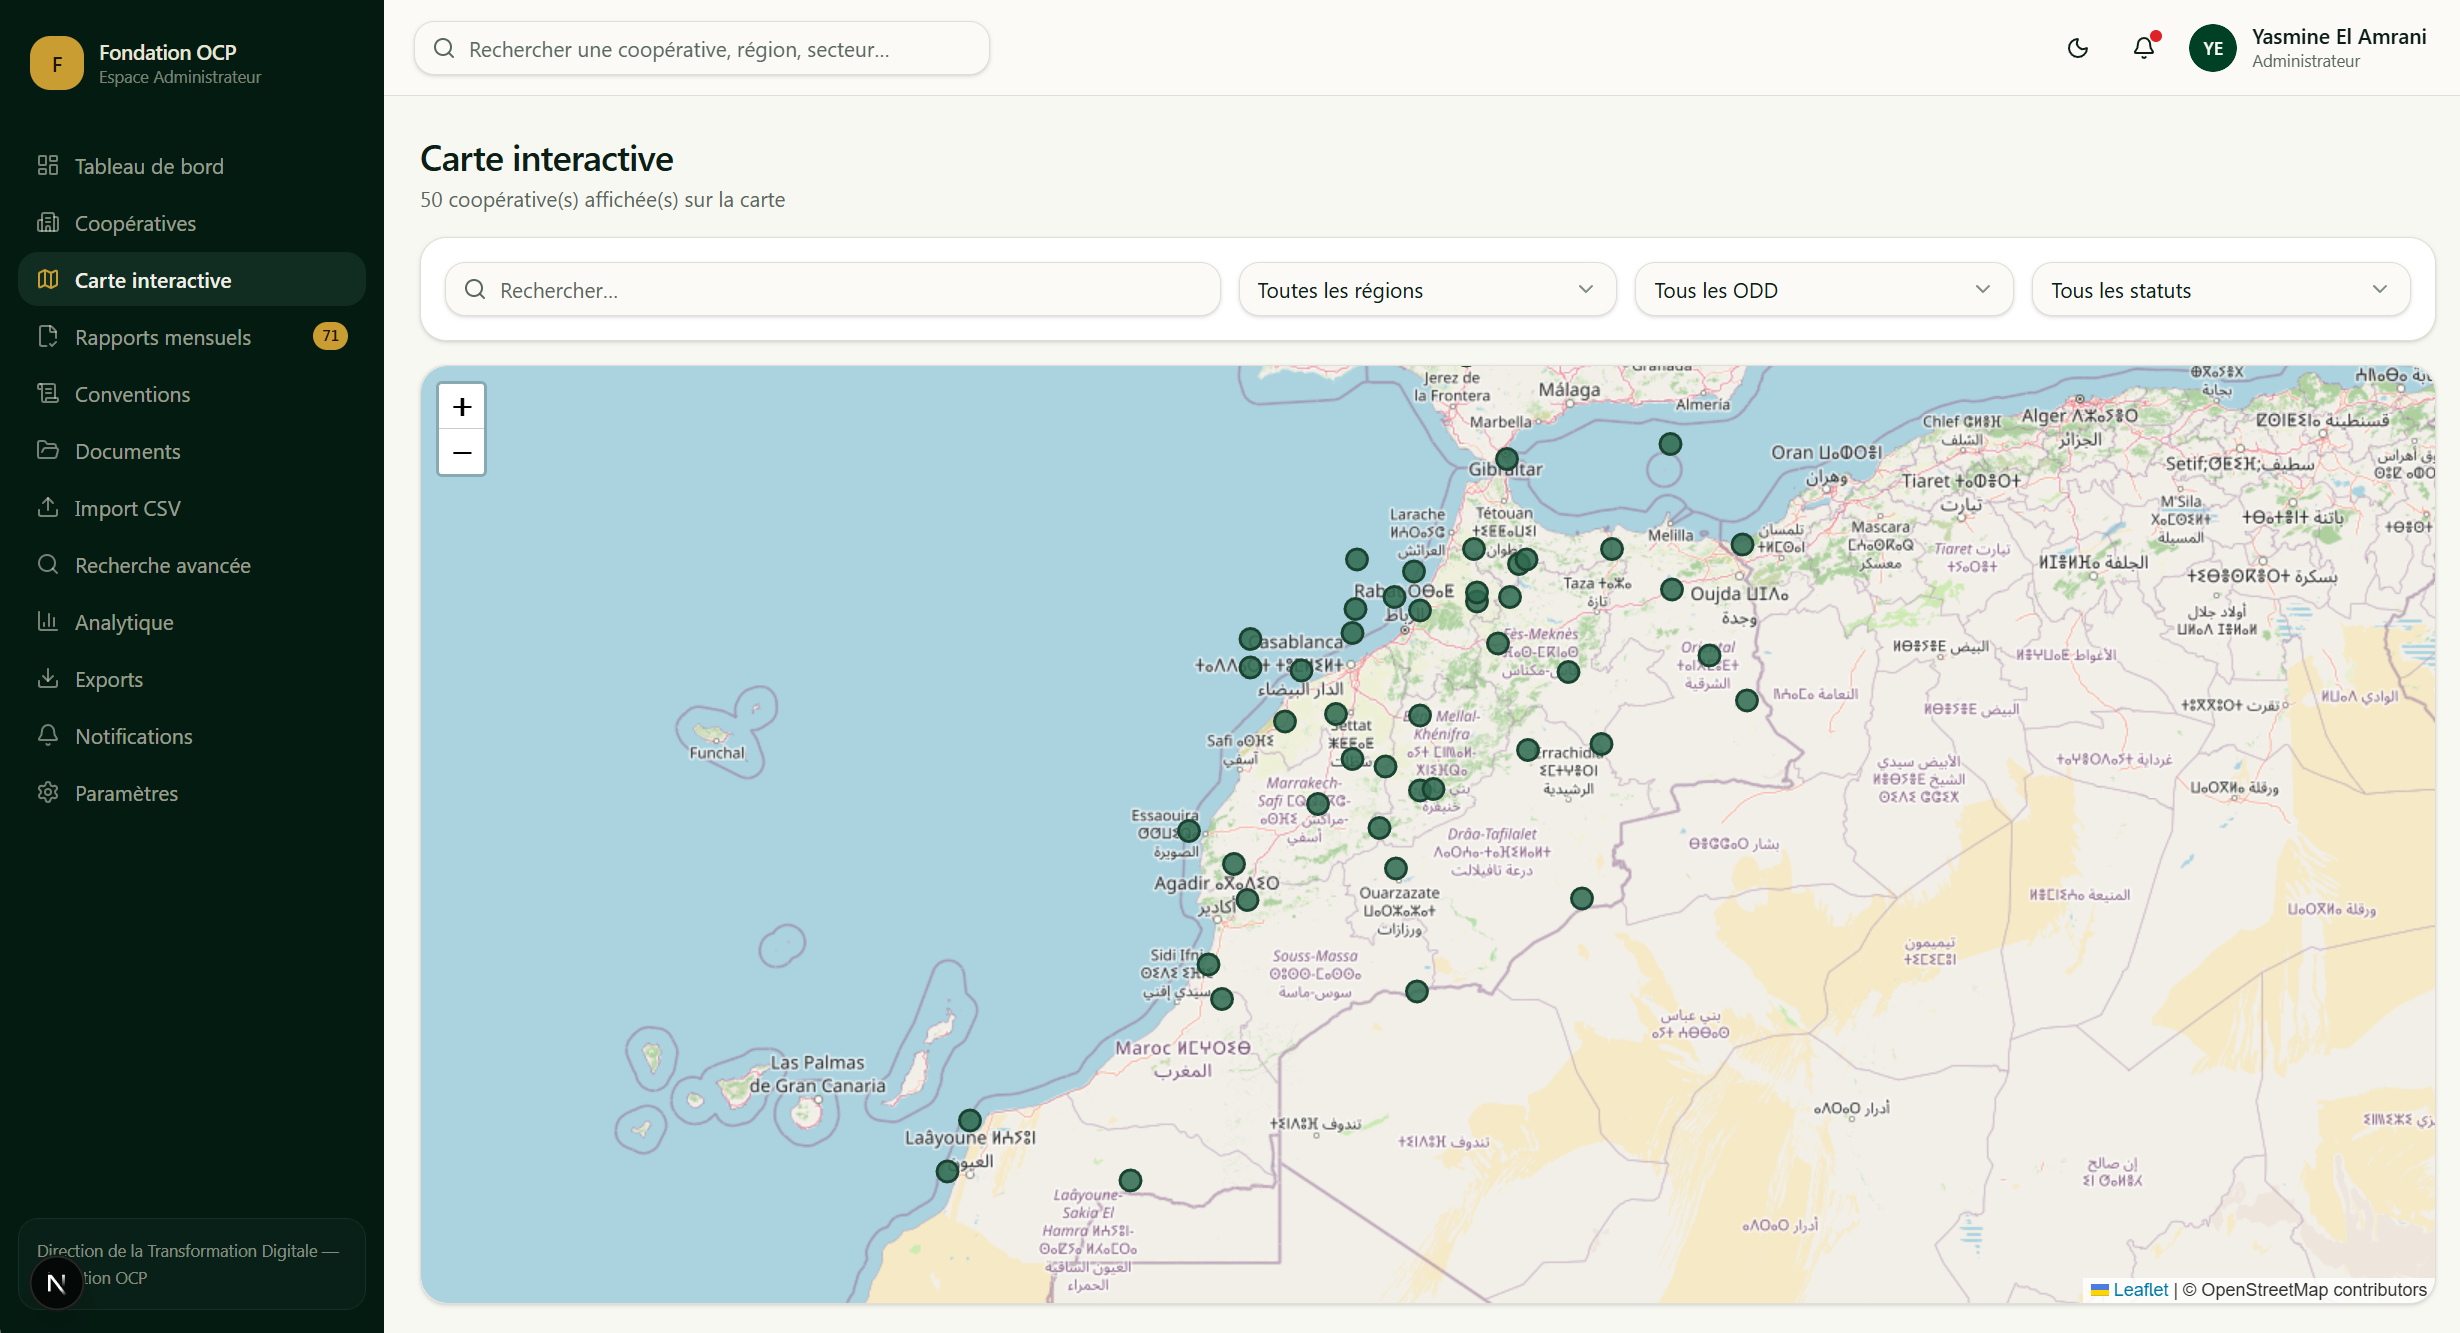
\includegraphics[width=0.90\textwidth]{figures/screenshots/mvp/04_mvp_carte_interactive.png}
\caption{Cartographie interactive nationale des coopératives et bénéficiaires}
\label{fig:mvp_04_map}
\end{figure}

L'interface propose des filtres dynamiques par région et secteur d'activité, affichant des infobulles détaillées lors du survol ou du clic sur chaque point géographique.

\subsection{Suivi et circuit de validation des rapports d'activité mensuels}

Le module de gestion des rapports mensuels (figure \ref{fig:mvp_05_reports}) dématérialise le workflow complet de reporting. Les coopératives y déclarent leurs activités et indicateurs mensuels, tandis que les équipes de la Fondation examinent les soumissions.

\begin{figure}[H]
\centering
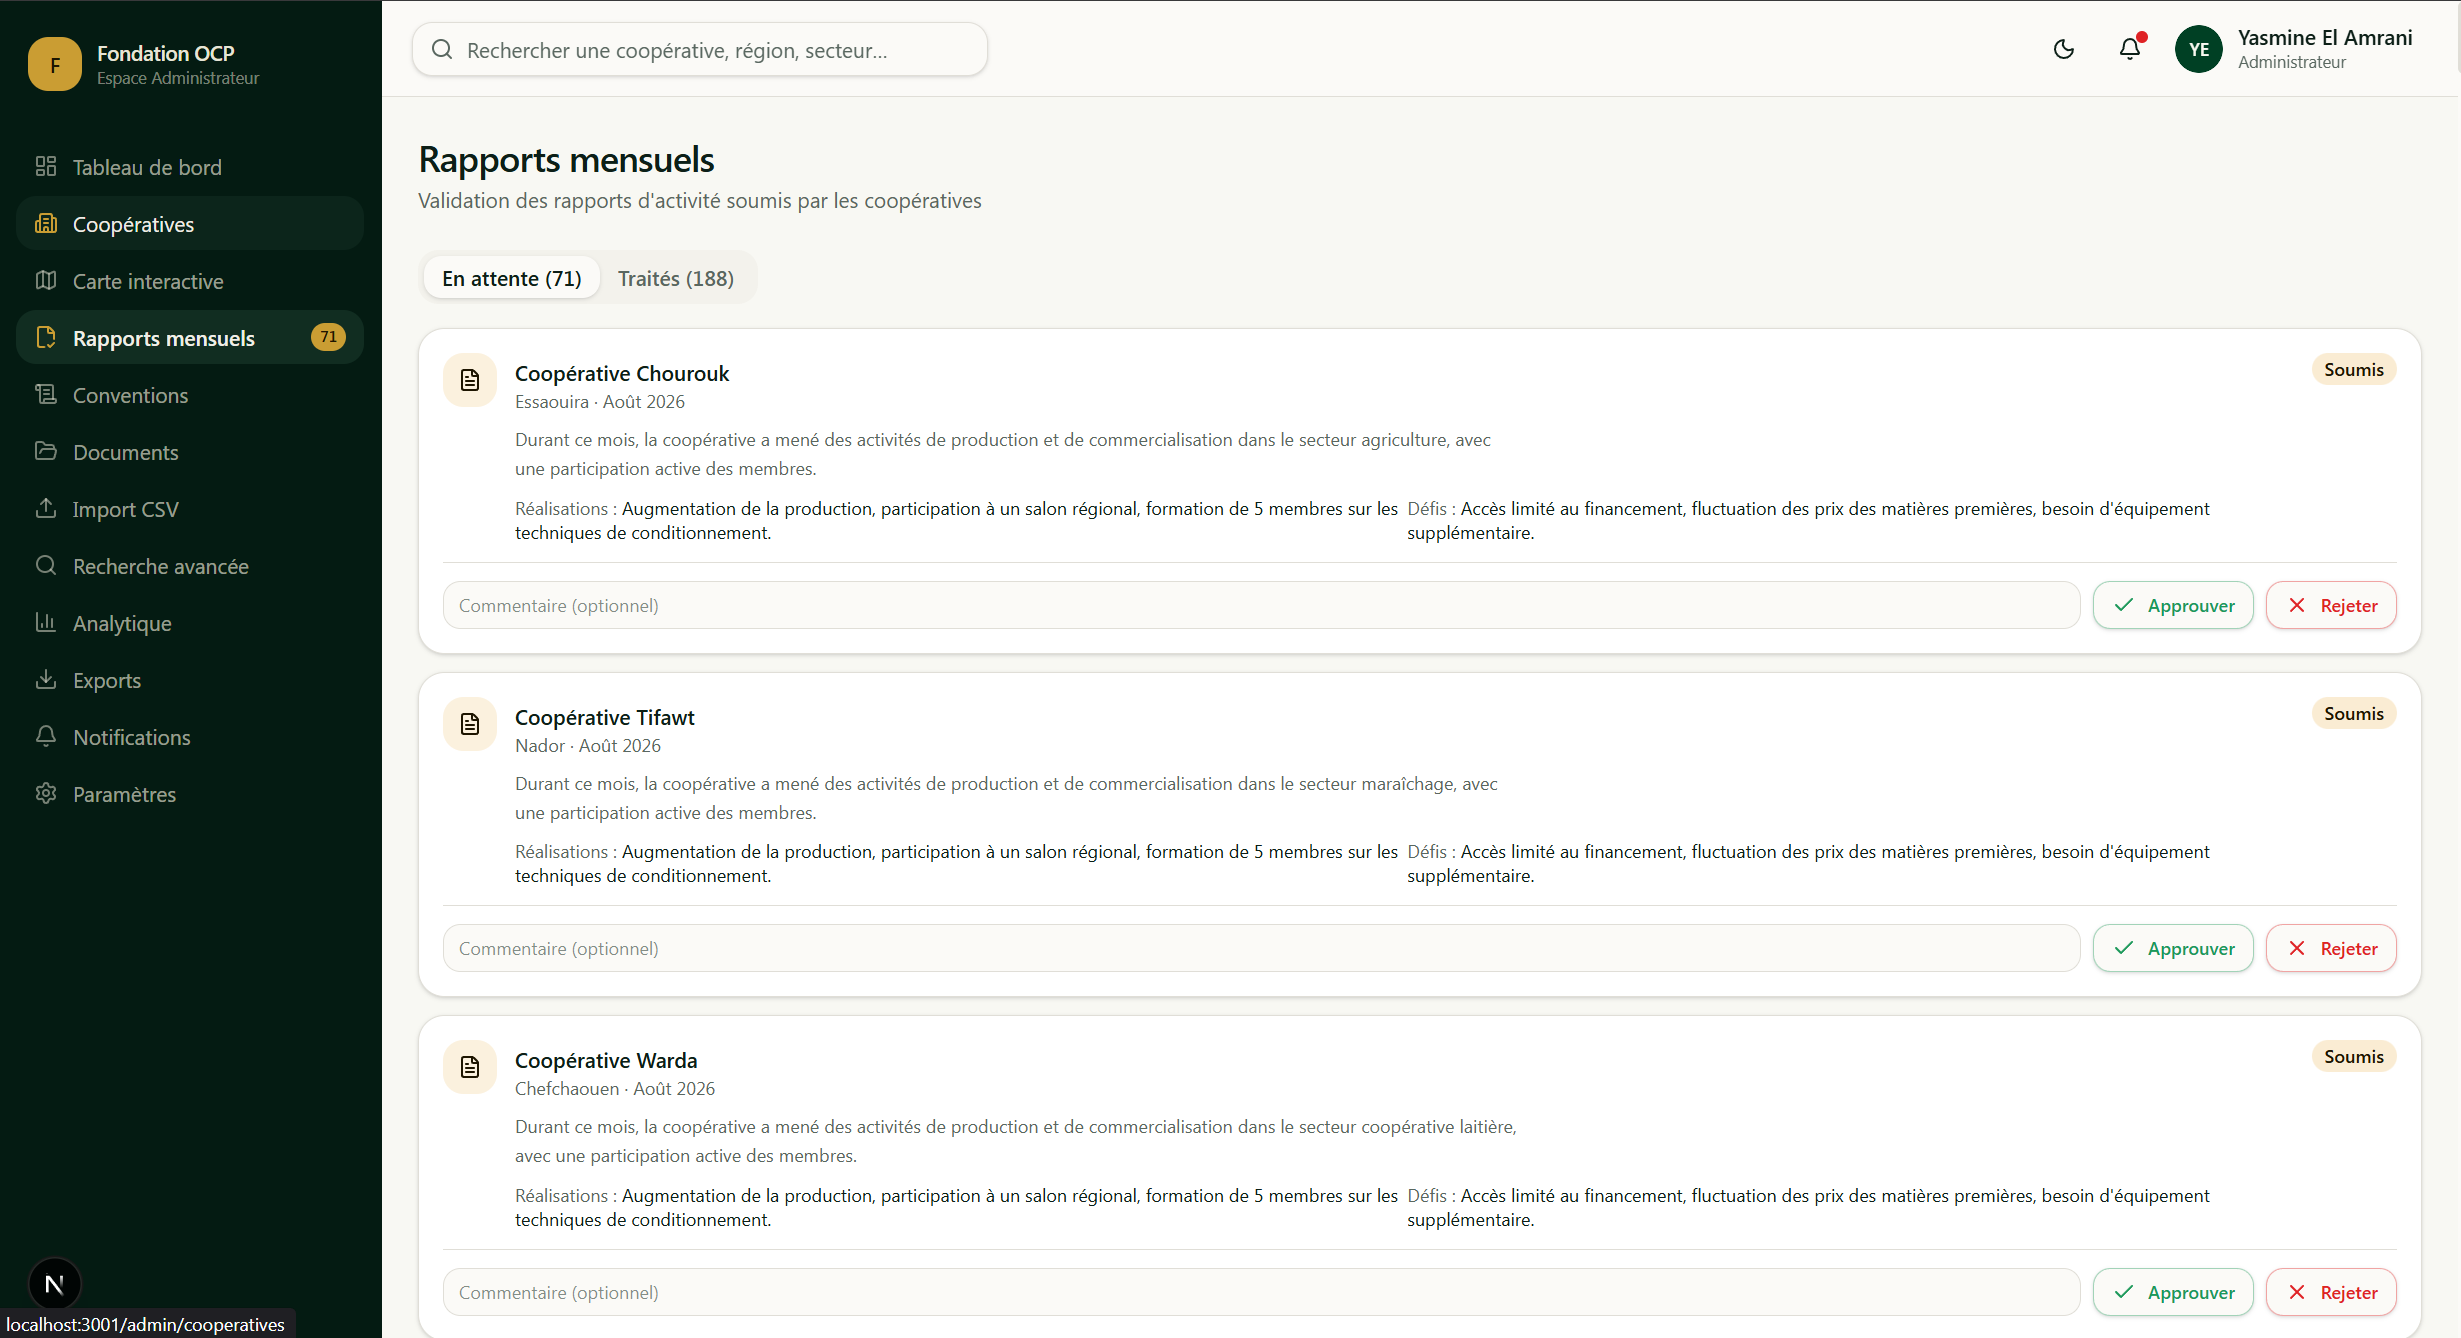
\includegraphics[width=0.90\textwidth]{figures/screenshots/mvp/05_mvp_rapports_mensuels.png}
\caption{Circuit de suivi, validation et rejet motivé des rapports mensuels}
\label{fig:mvp_05_reports}
\end{figure}

L'administrateur dispose des options de validation formelle ou de rejet avec obligation de renseigner un motif explicite, consigné dans le journal d'audit.

\subsection{Suivi des conventions de partenariat et gestion budgétaire}

L'interface de gestion des conventions (figure \ref{fig:mvp_06_conv}) assure le suivi administratif et financier des partenariats conclus entre la Fondation OCP et les coopératives.

\begin{figure}[H]
\centering
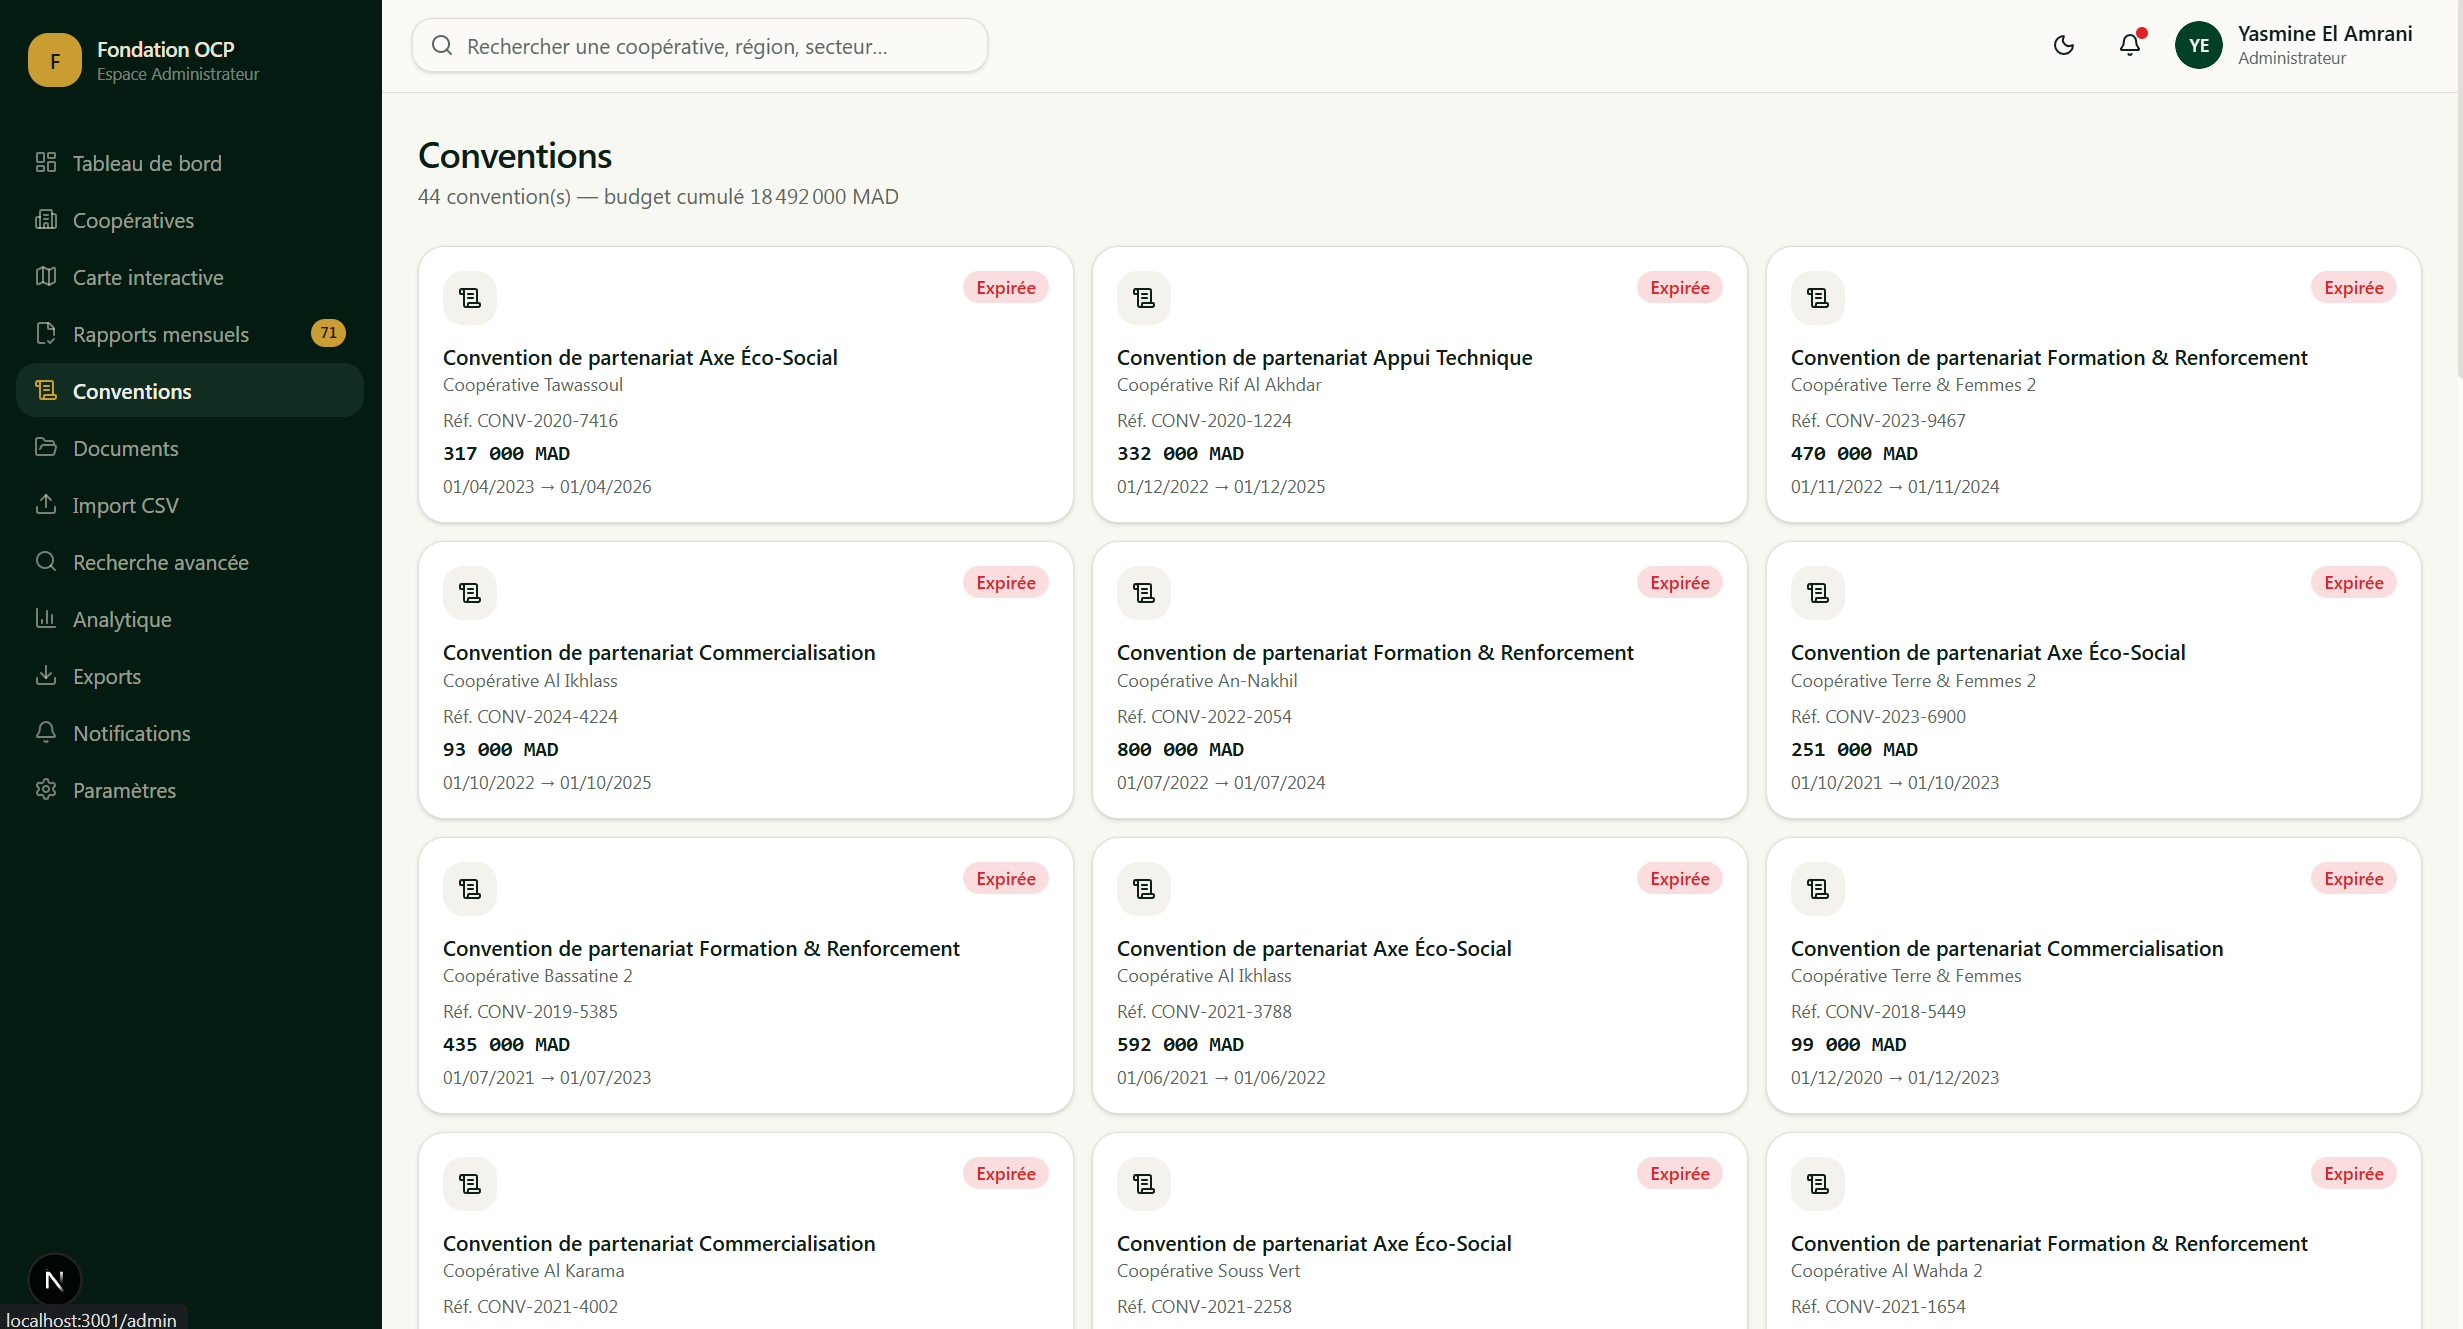
\includegraphics[width=0.90\textwidth]{figures/screenshots/mvp/06_mvp_conventions.png}
\caption{Gestion des conventions de partenariat et suivi des engagements budgétaires}
\label{fig:mvp_06_conv}
\end{figure}

Elle permet de suivre les dates d'effet, les échéances, les montants engagés, les budgets décaissés et les pièces contractuelles associées.

\subsection{Gestion électronique de documents (GED) et pièces justificatives}

Le module documentaire GED (figure \ref{fig:mvp_07_ged}) centralise le dépôt, le stockage sécurisé et la validation des pièces justificatives (statuts légaux, PV d'assemblées générales, listes d'émargement, attestations de versement).

\begin{figure}[H]
\centering
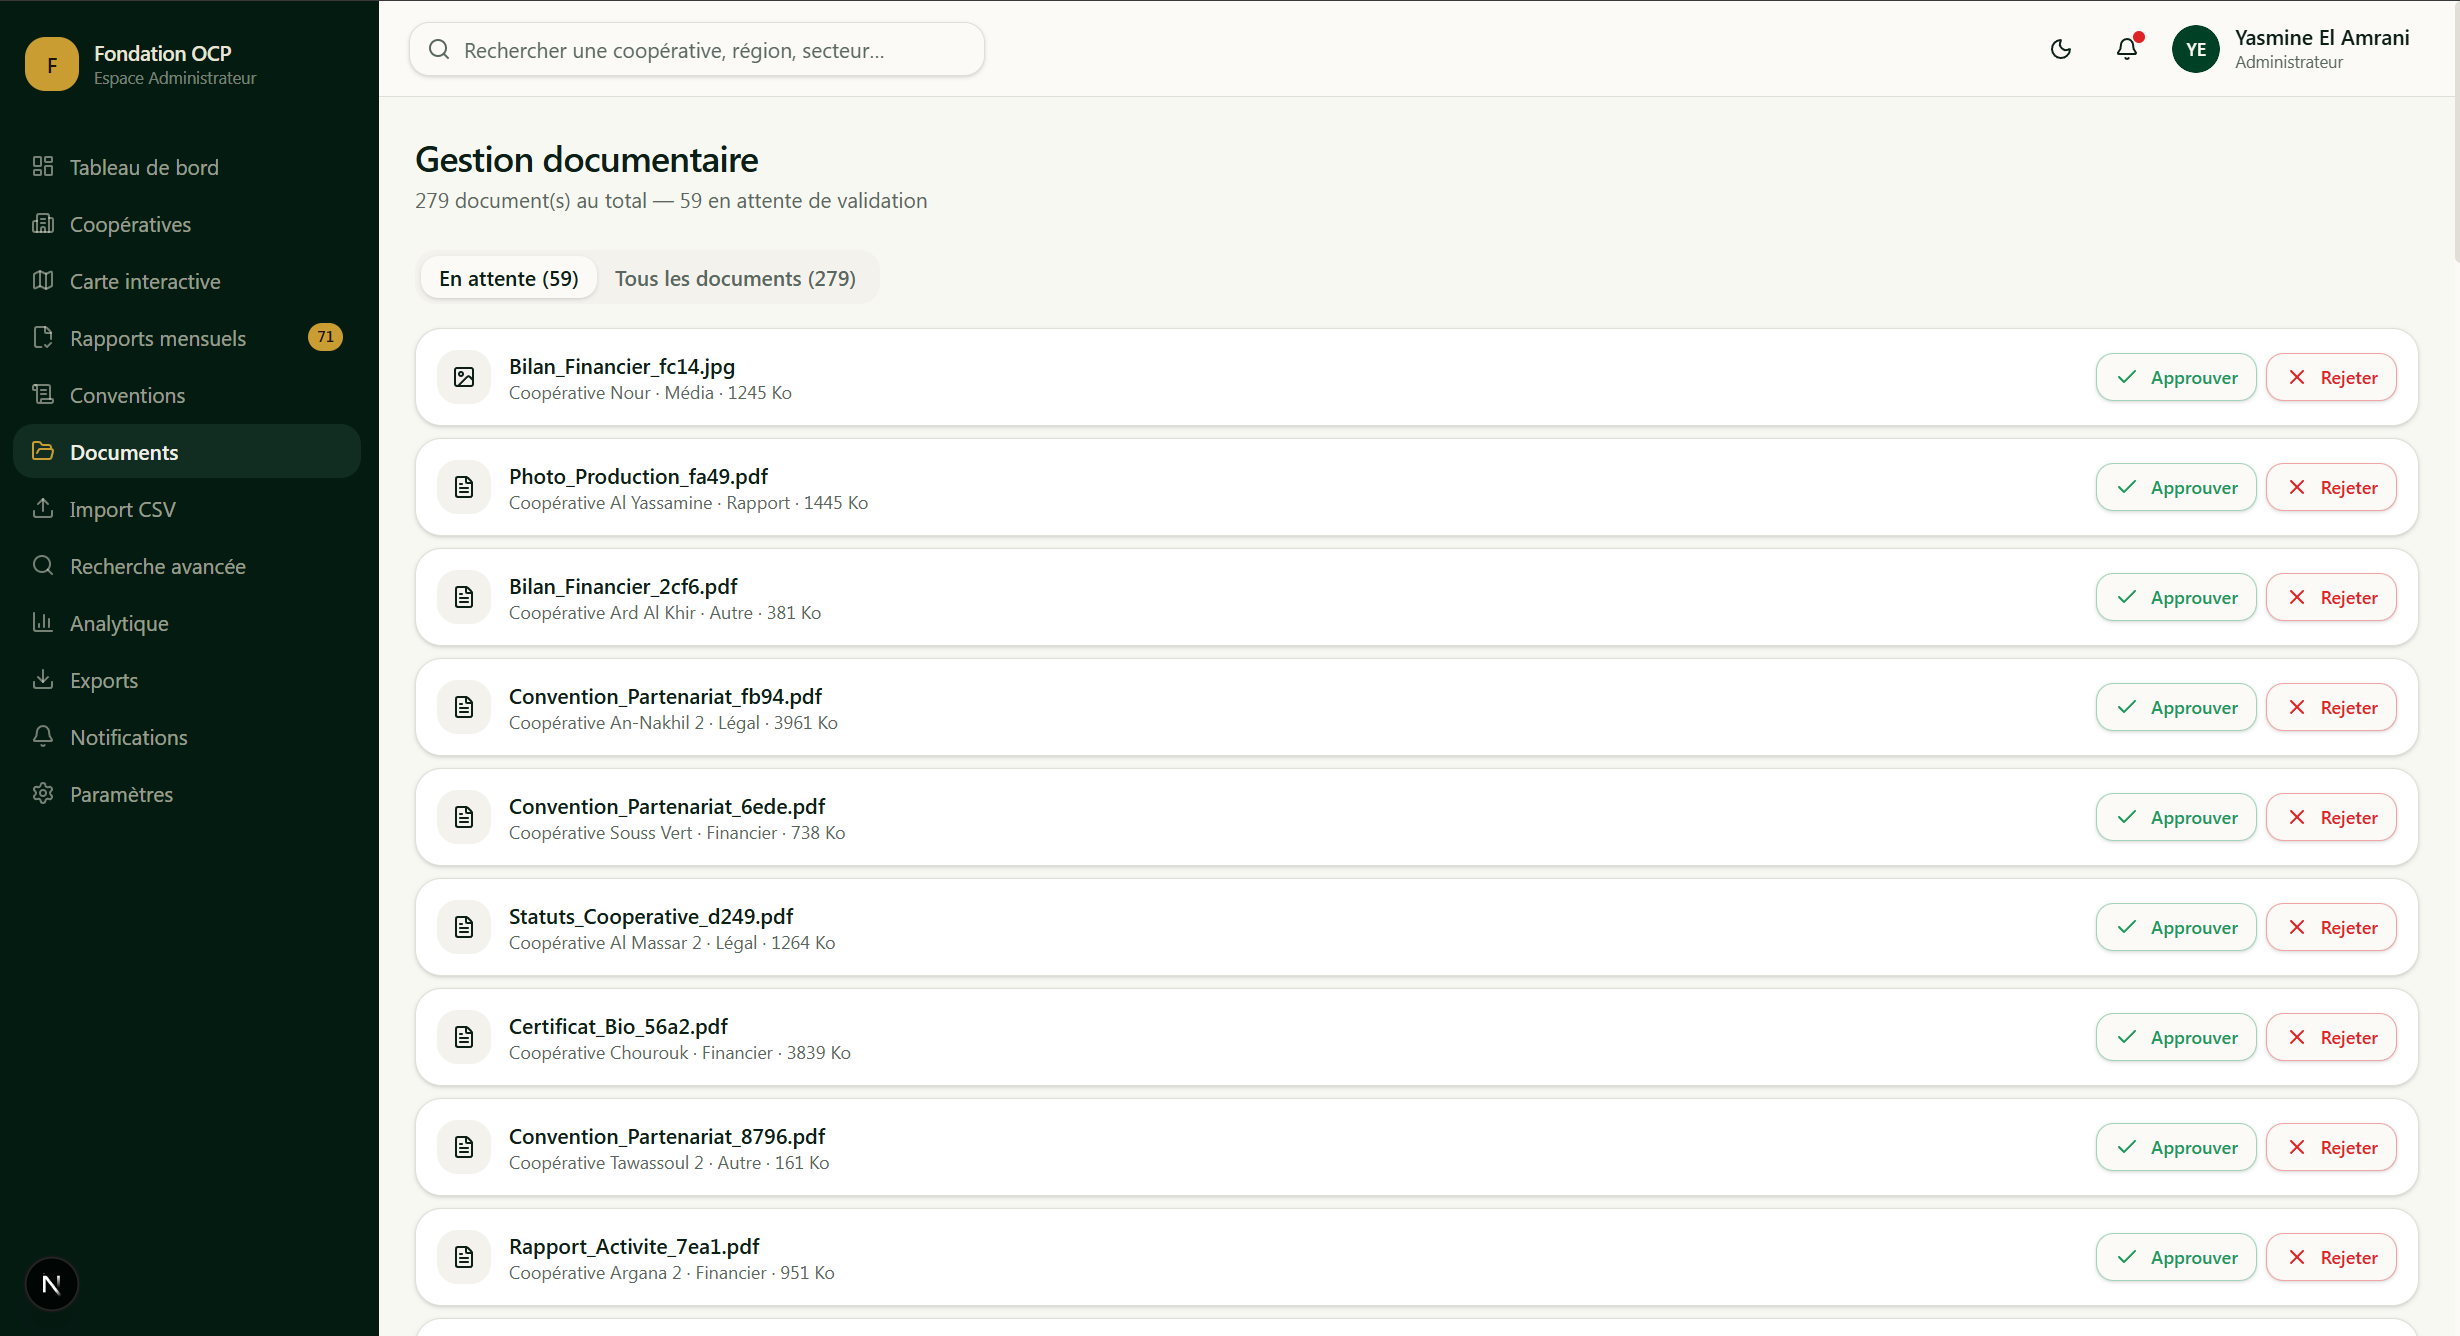
\includegraphics[width=0.90\textwidth]{figures/screenshots/mvp/07_mvp_documents.png}
\caption{Module de Gestion Électronique des Documents (GED) et validation des pièces}
\label{fig:mvp_07_ged}
\end{figure}

Le système applique des contrôles stricts sur les types de fichiers (PDF, images), vérifie l'absence de scripts malveillants et garantit l'intégrité des pièces déposées.

\subsection{Importation massive des données de coopératives par fichier CSV}

Pour faciliter l'initialisation du réseau ou la mise à jour périodique par lots, le MVP intègre un moteur d'importation de fichiers CSV (figure \ref{fig:mvp_08_import}).

\begin{figure}[H]
\centering
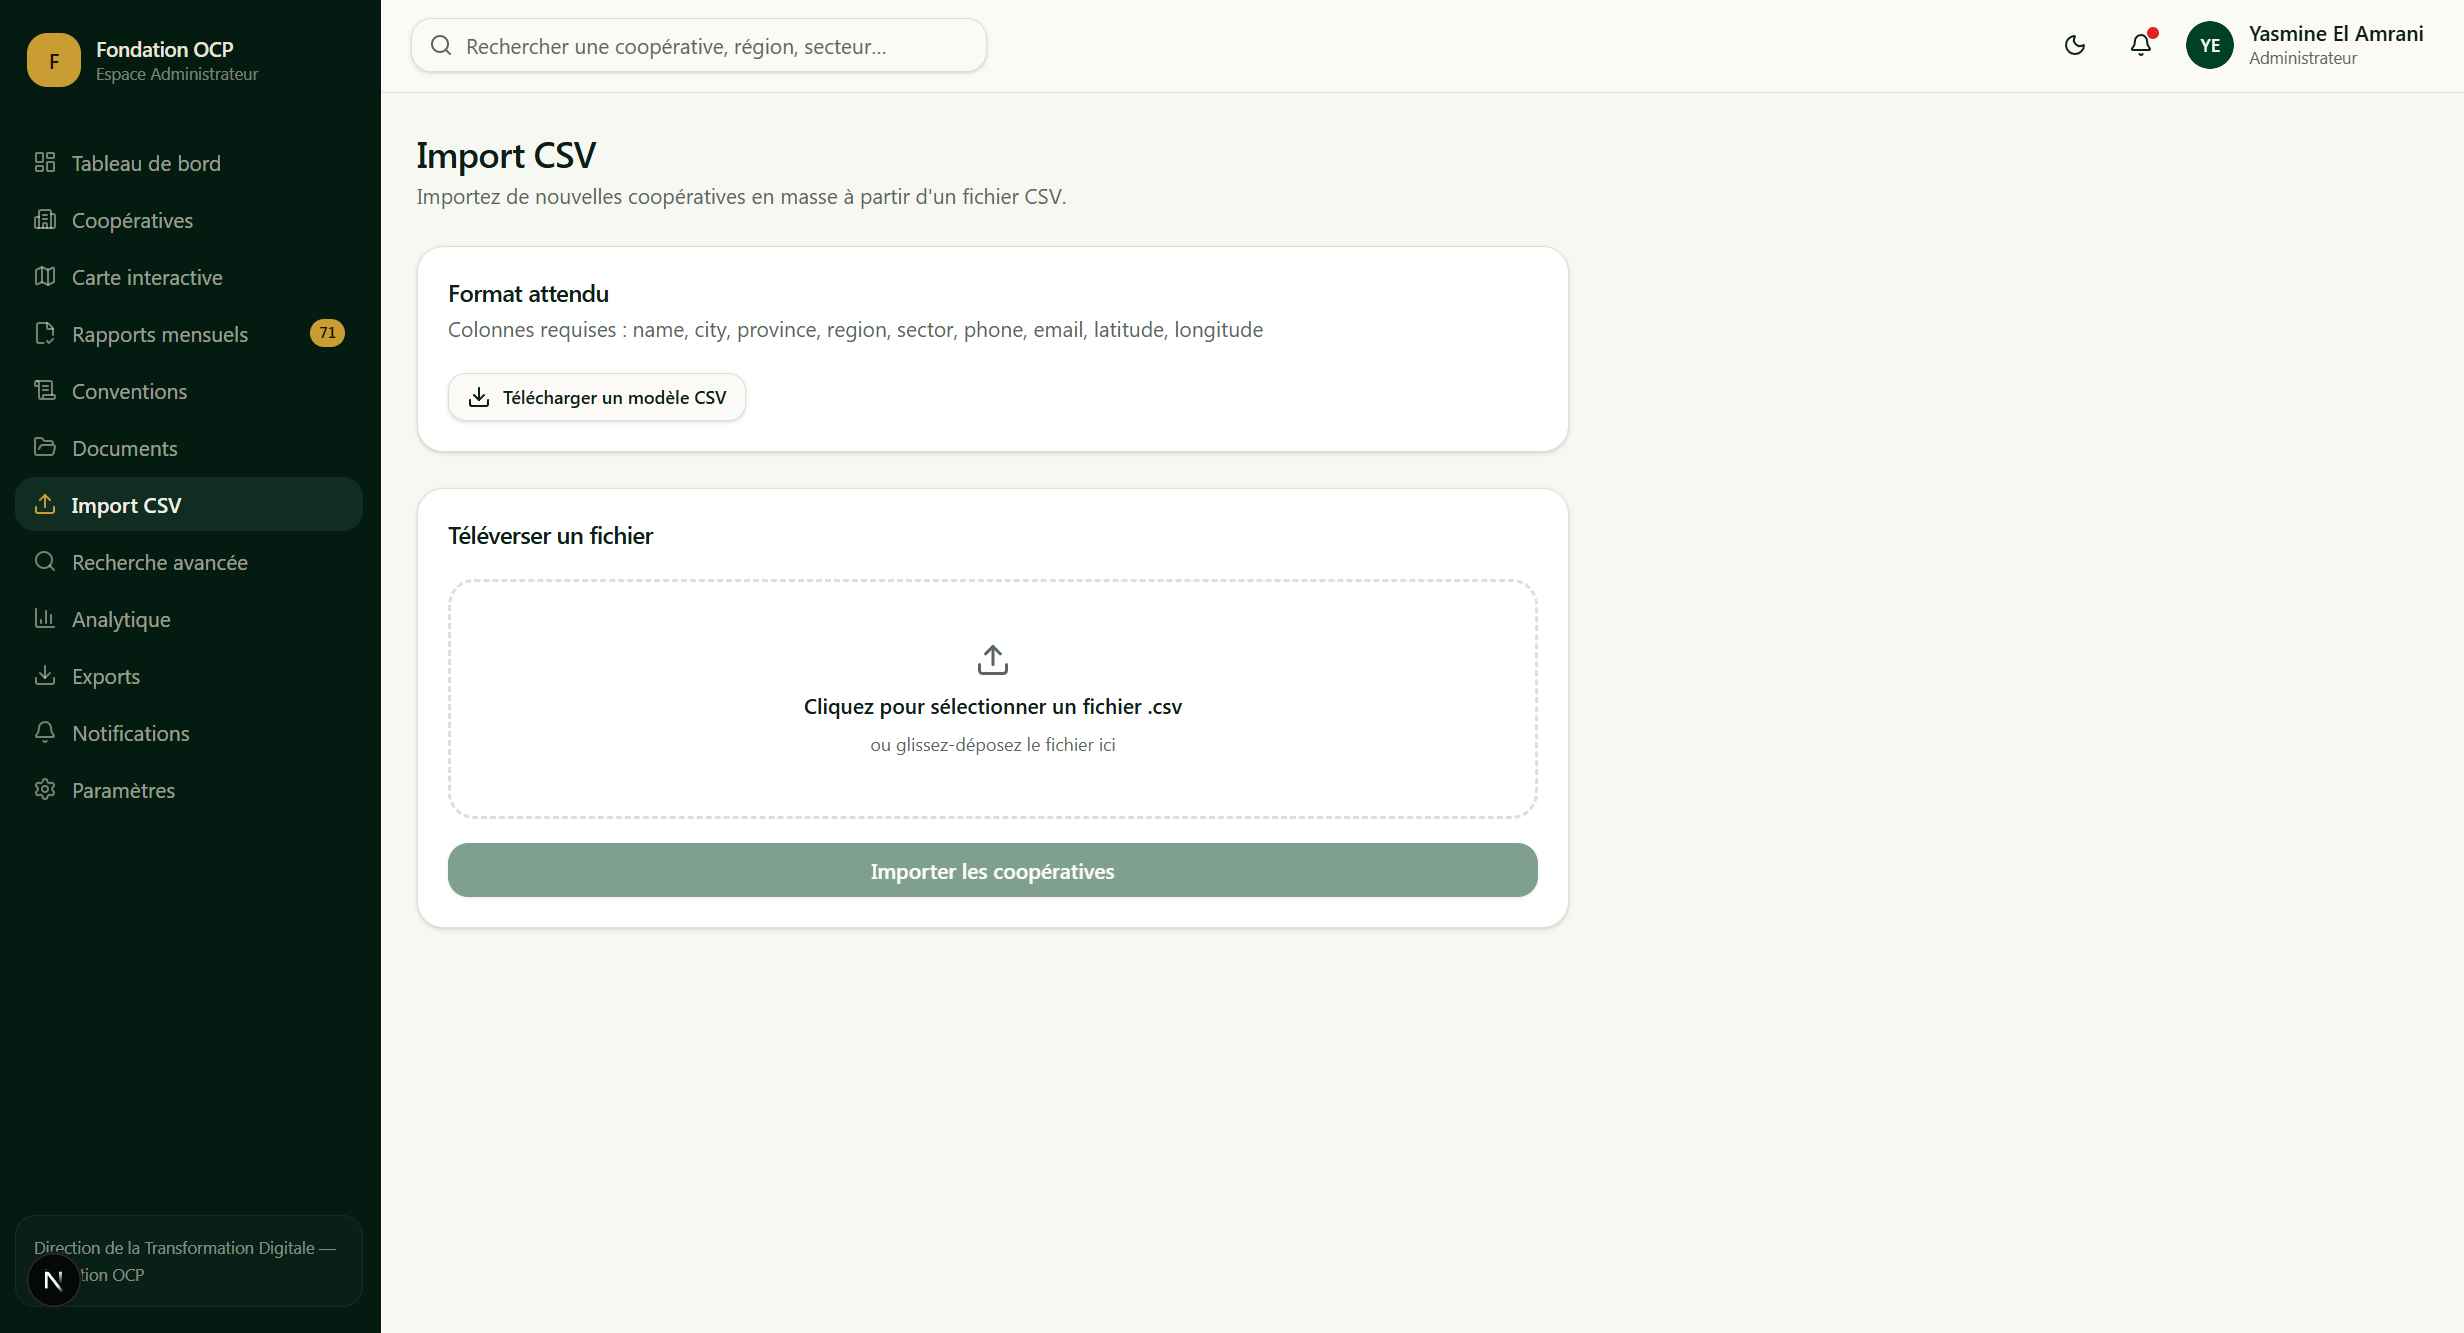
\includegraphics[width=0.90\textwidth]{figures/screenshots/mvp/08_mvp_import_csv.png}
\caption{Interface d'importation massive des coopératives via fichier CSV}
\label{fig:mvp_08_import}
\end{figure}

Ce module propose un modèle de données type, analyse les lignes importées, détecte les anomalies de format et valide l'intégrité avant insertion en base.

\subsection{Moteur de recherche multicritère avancée et filtrage dynamique}

L'interface de recherche avancée (figure \ref{fig:mvp_09_search}) permet aux administrateurs de croiser de multiples critères de recherche (région, secteur, plage de bénéficiaires, conformité des déclarations, statut de convention).

\begin{figure}[H]
\centering
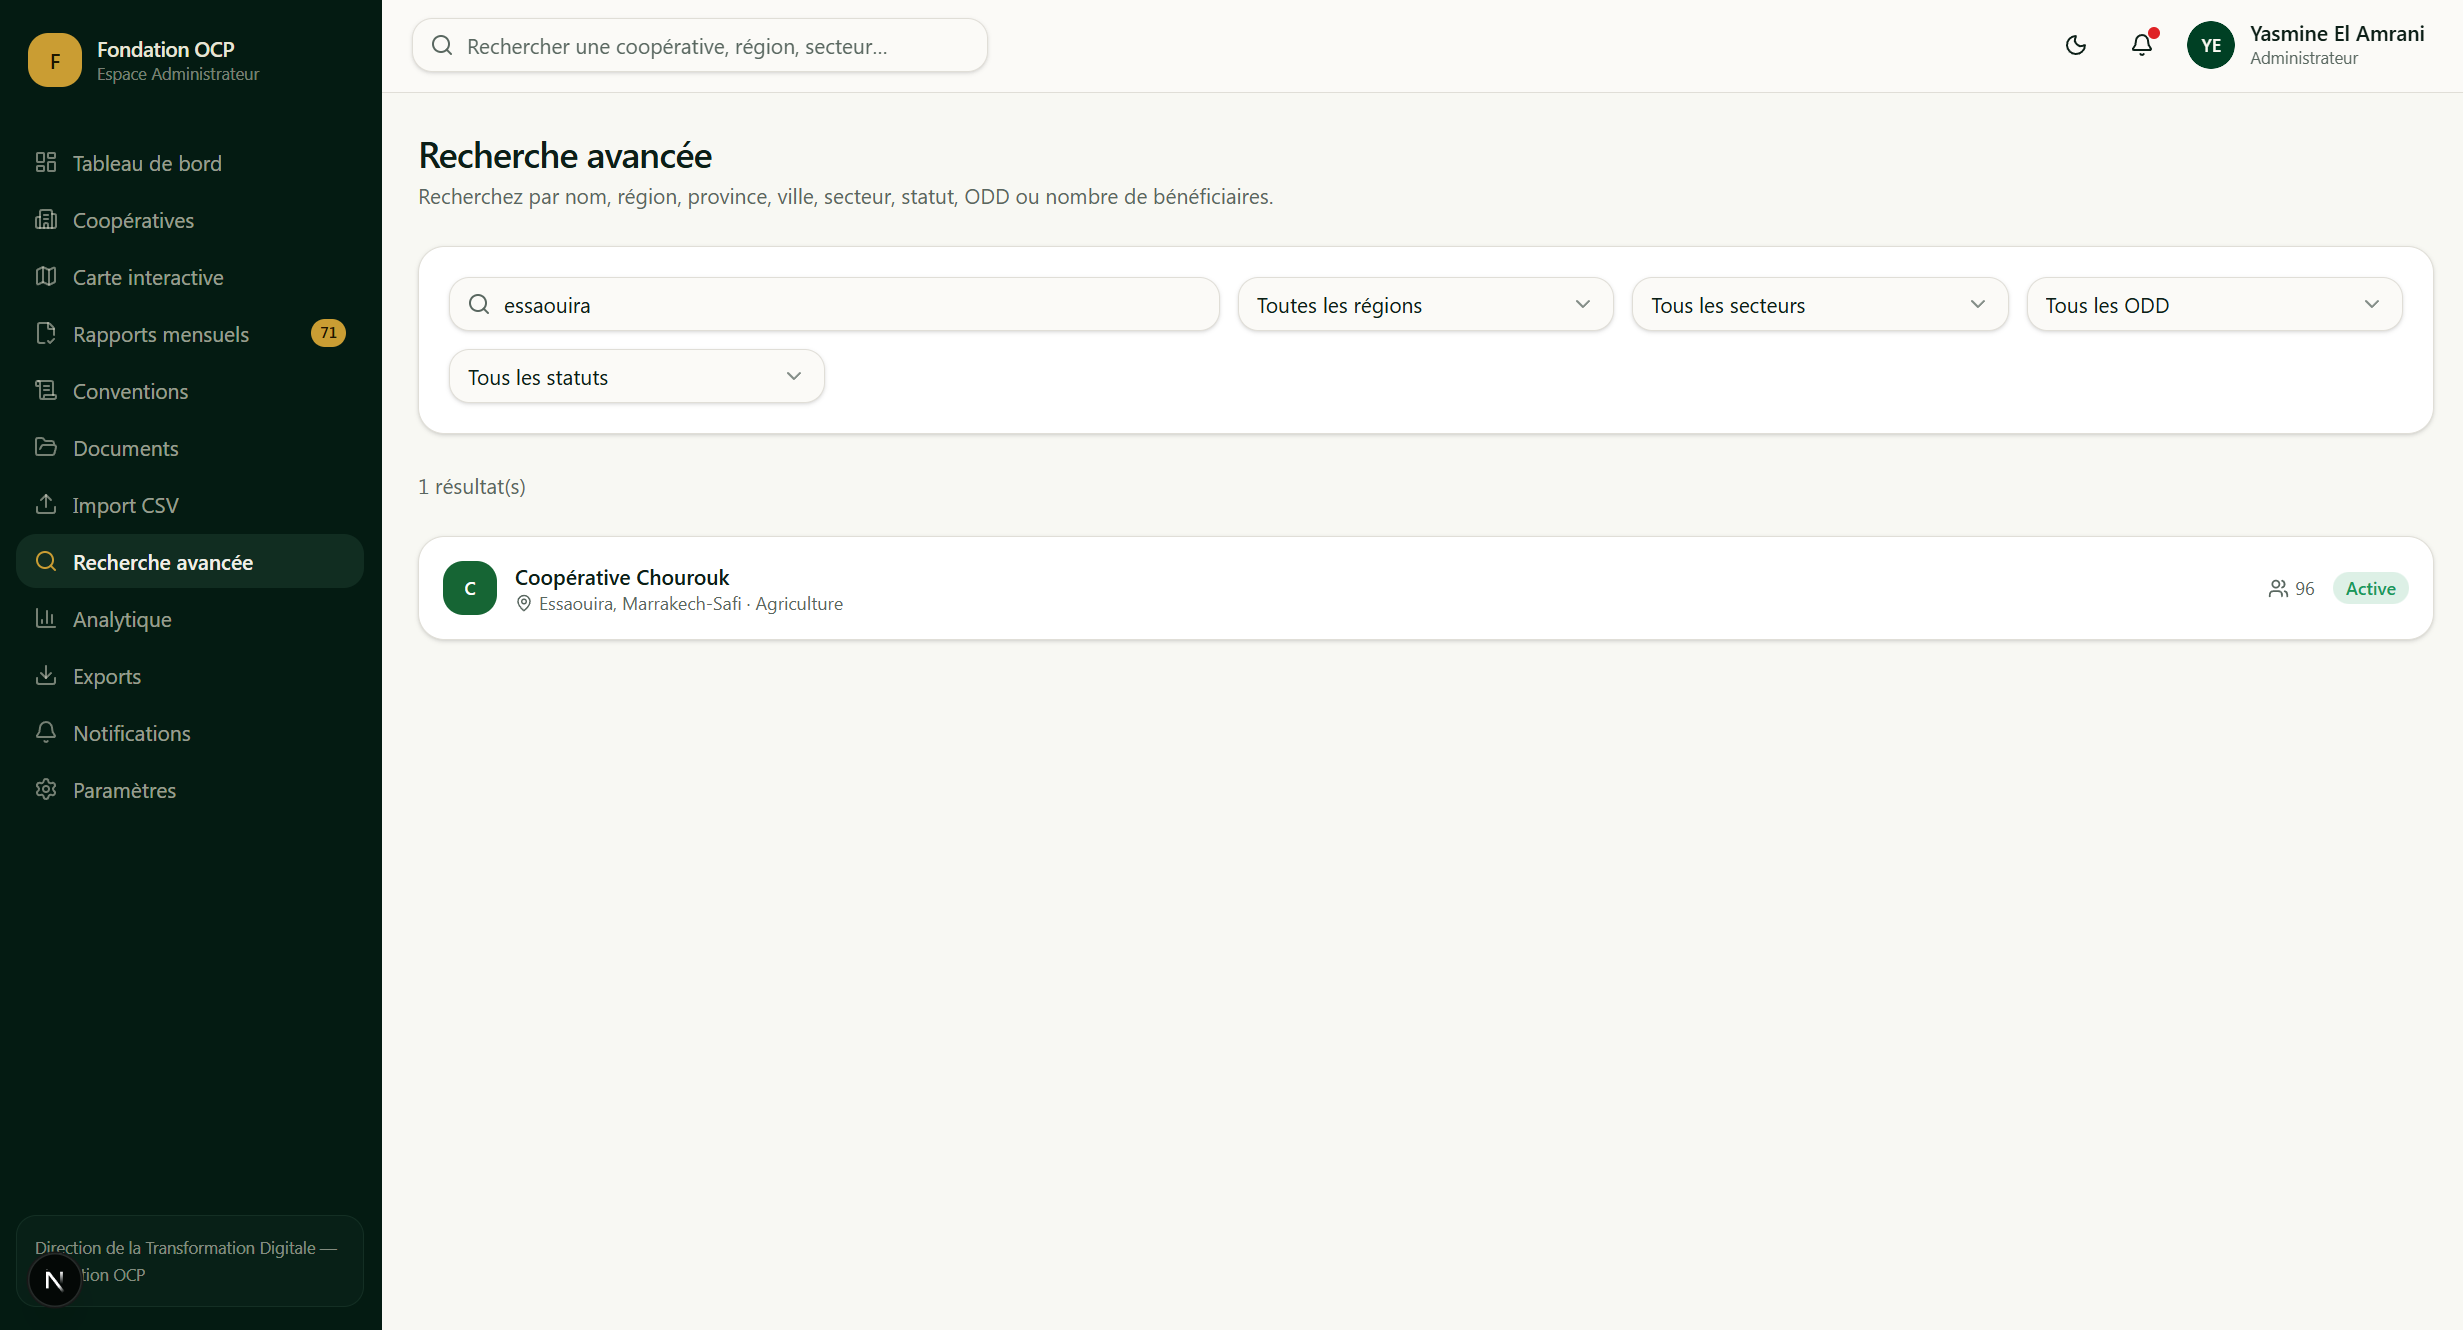
\includegraphics[width=0.90\textwidth]{figures/screenshots/mvp/09_mvp_recherche_avancee.png}
\caption{Moteur de recherche multicritère avancée et filtrage combiné}
\label{fig:mvp_09_search}
\end{figure}

Cette fonctionnalité répond au besoin d'audit et d'extraction ciblée exprimé par les directions métiers de la Fondation.

\subsection{Tableau de bord analytique avancé (Parité, ESG et ODD)}

L'espace analytique approfondi (figure \ref{fig:mvp_10_analytics}) fournit des visualisations détaillées dédiées aux indicateurs d'impact durable : ratio de parité femmes/hommes, inclusion des jeunes ruraux, personnes en situation de handicap et alignement avec les objectifs ESG.

\begin{figure}[H]
\centering
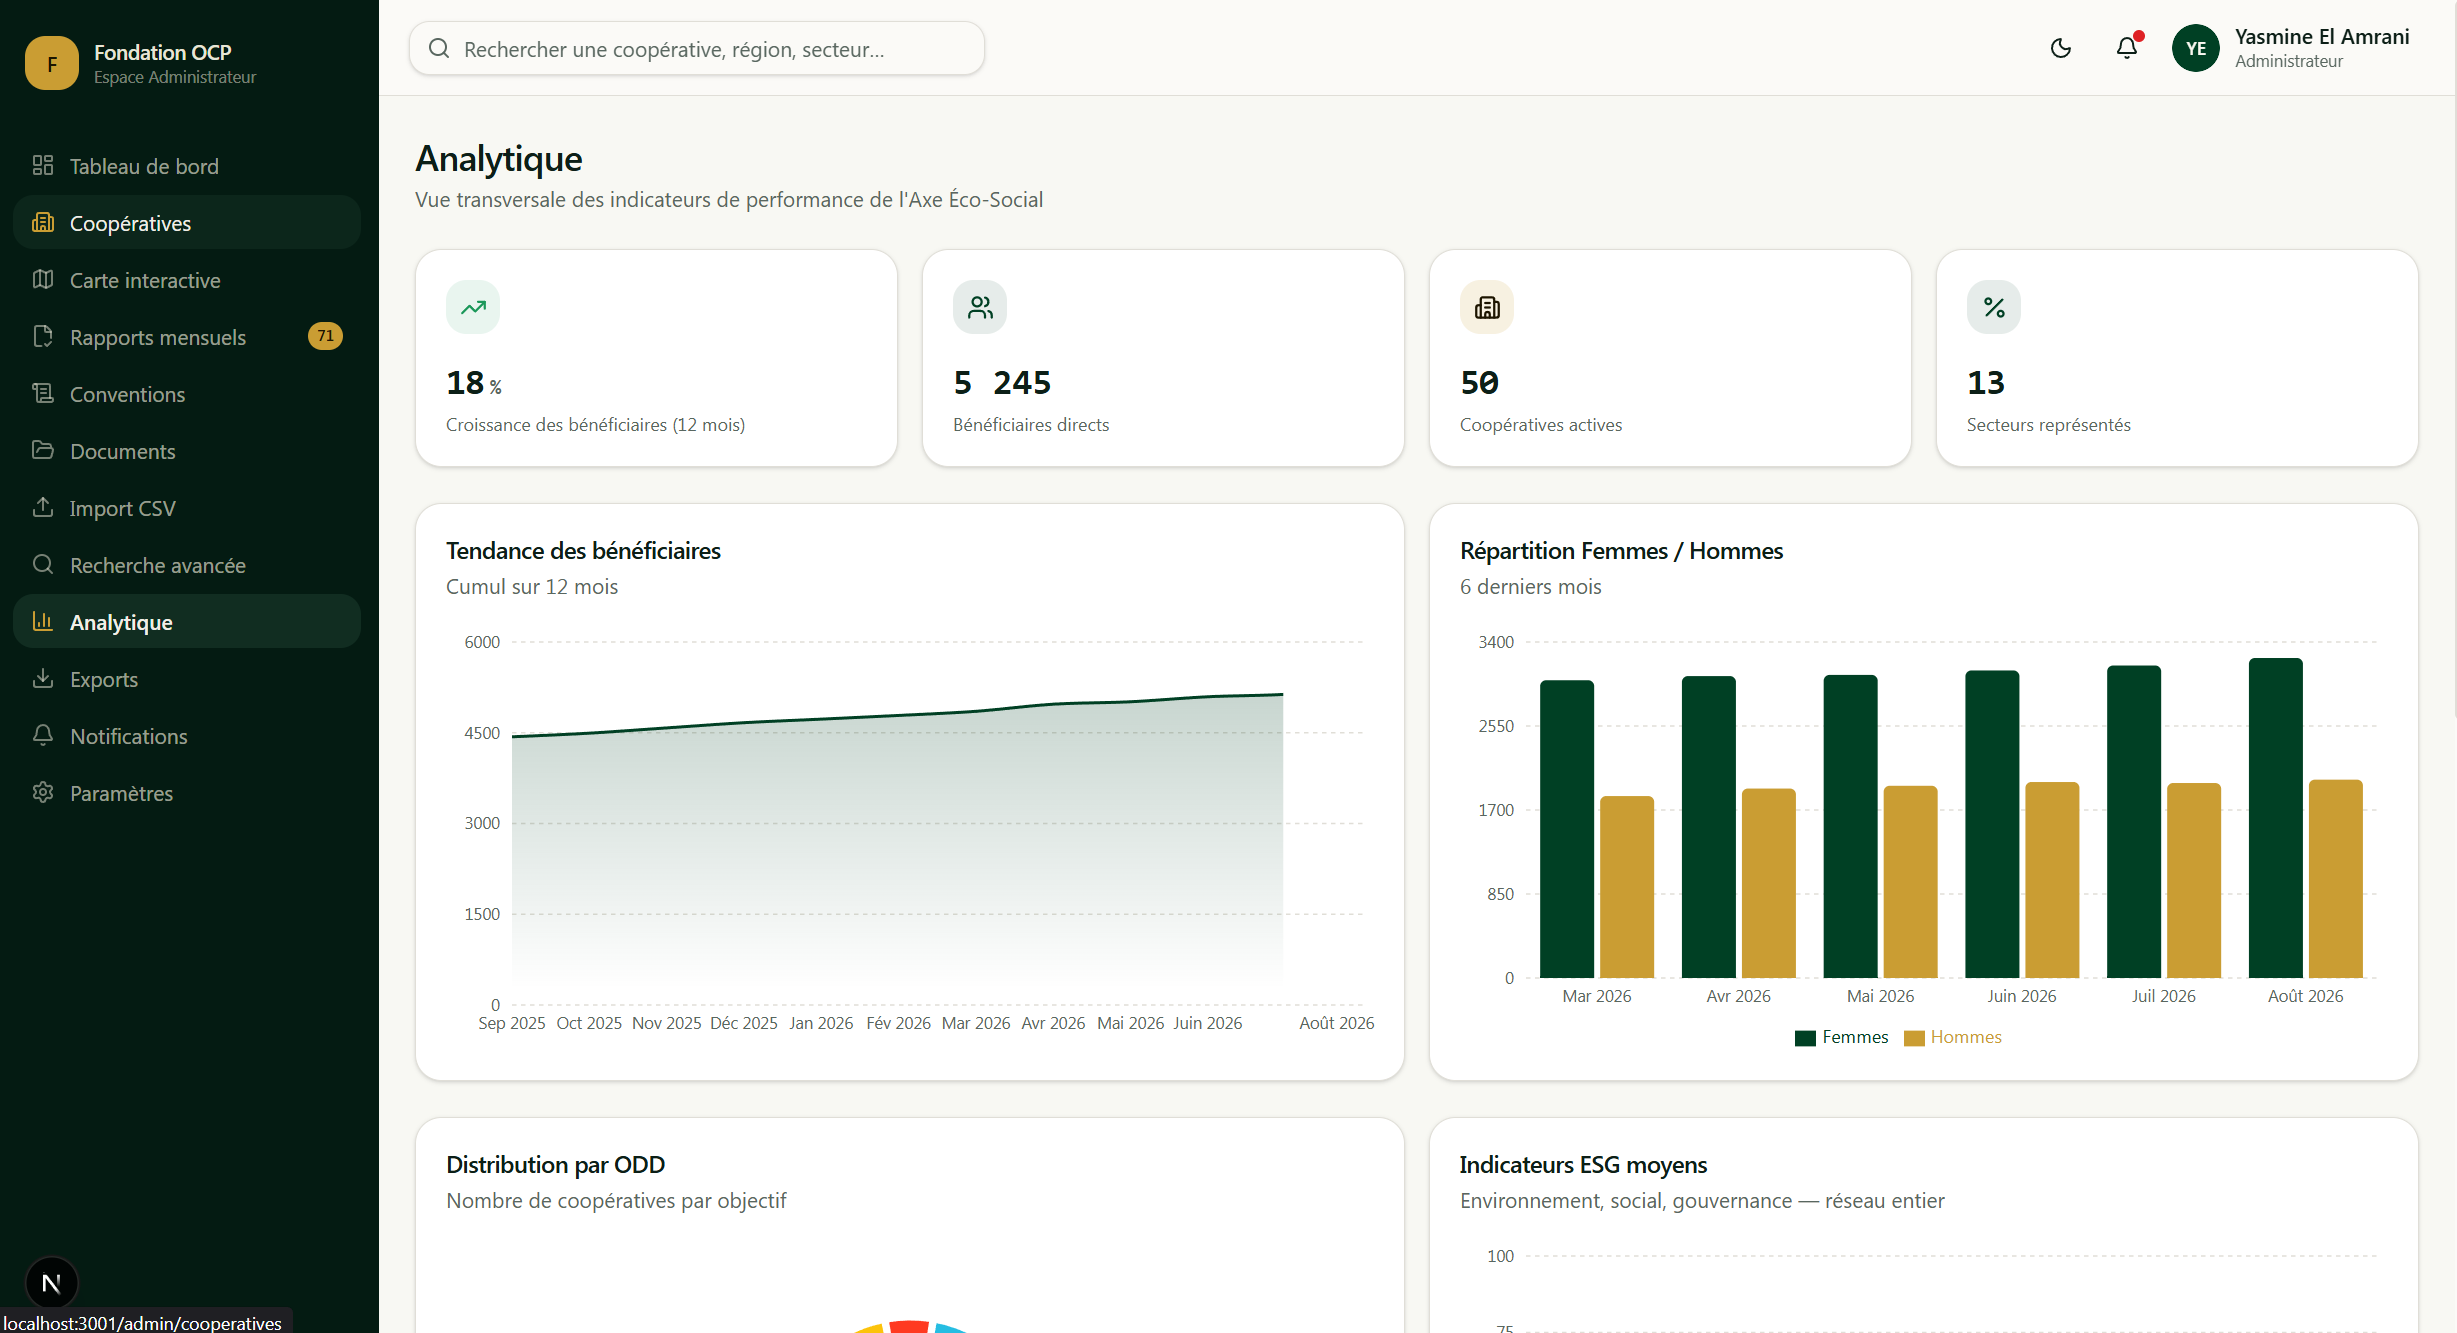
\includegraphics[width=0.90\textwidth]{figures/screenshots/mvp/10_mvp_analytique.png}
\caption{Tableau de bord analytique avancé : parité de genre, impact ESG et ODD}
\label{fig:mvp_10_analytics}
\end{figure}

\subsection{Module d'exportation multi-format des données consolidées}

Le module d'exportation (figure \ref{fig:mvp_11_export}) permet de générer des extractions des données globales ou filtrées sous différents formats normalisés : CSV, tableur Excel (.xlsx) et rapport de synthèse au format PDF.

\begin{figure}[H]
\centering
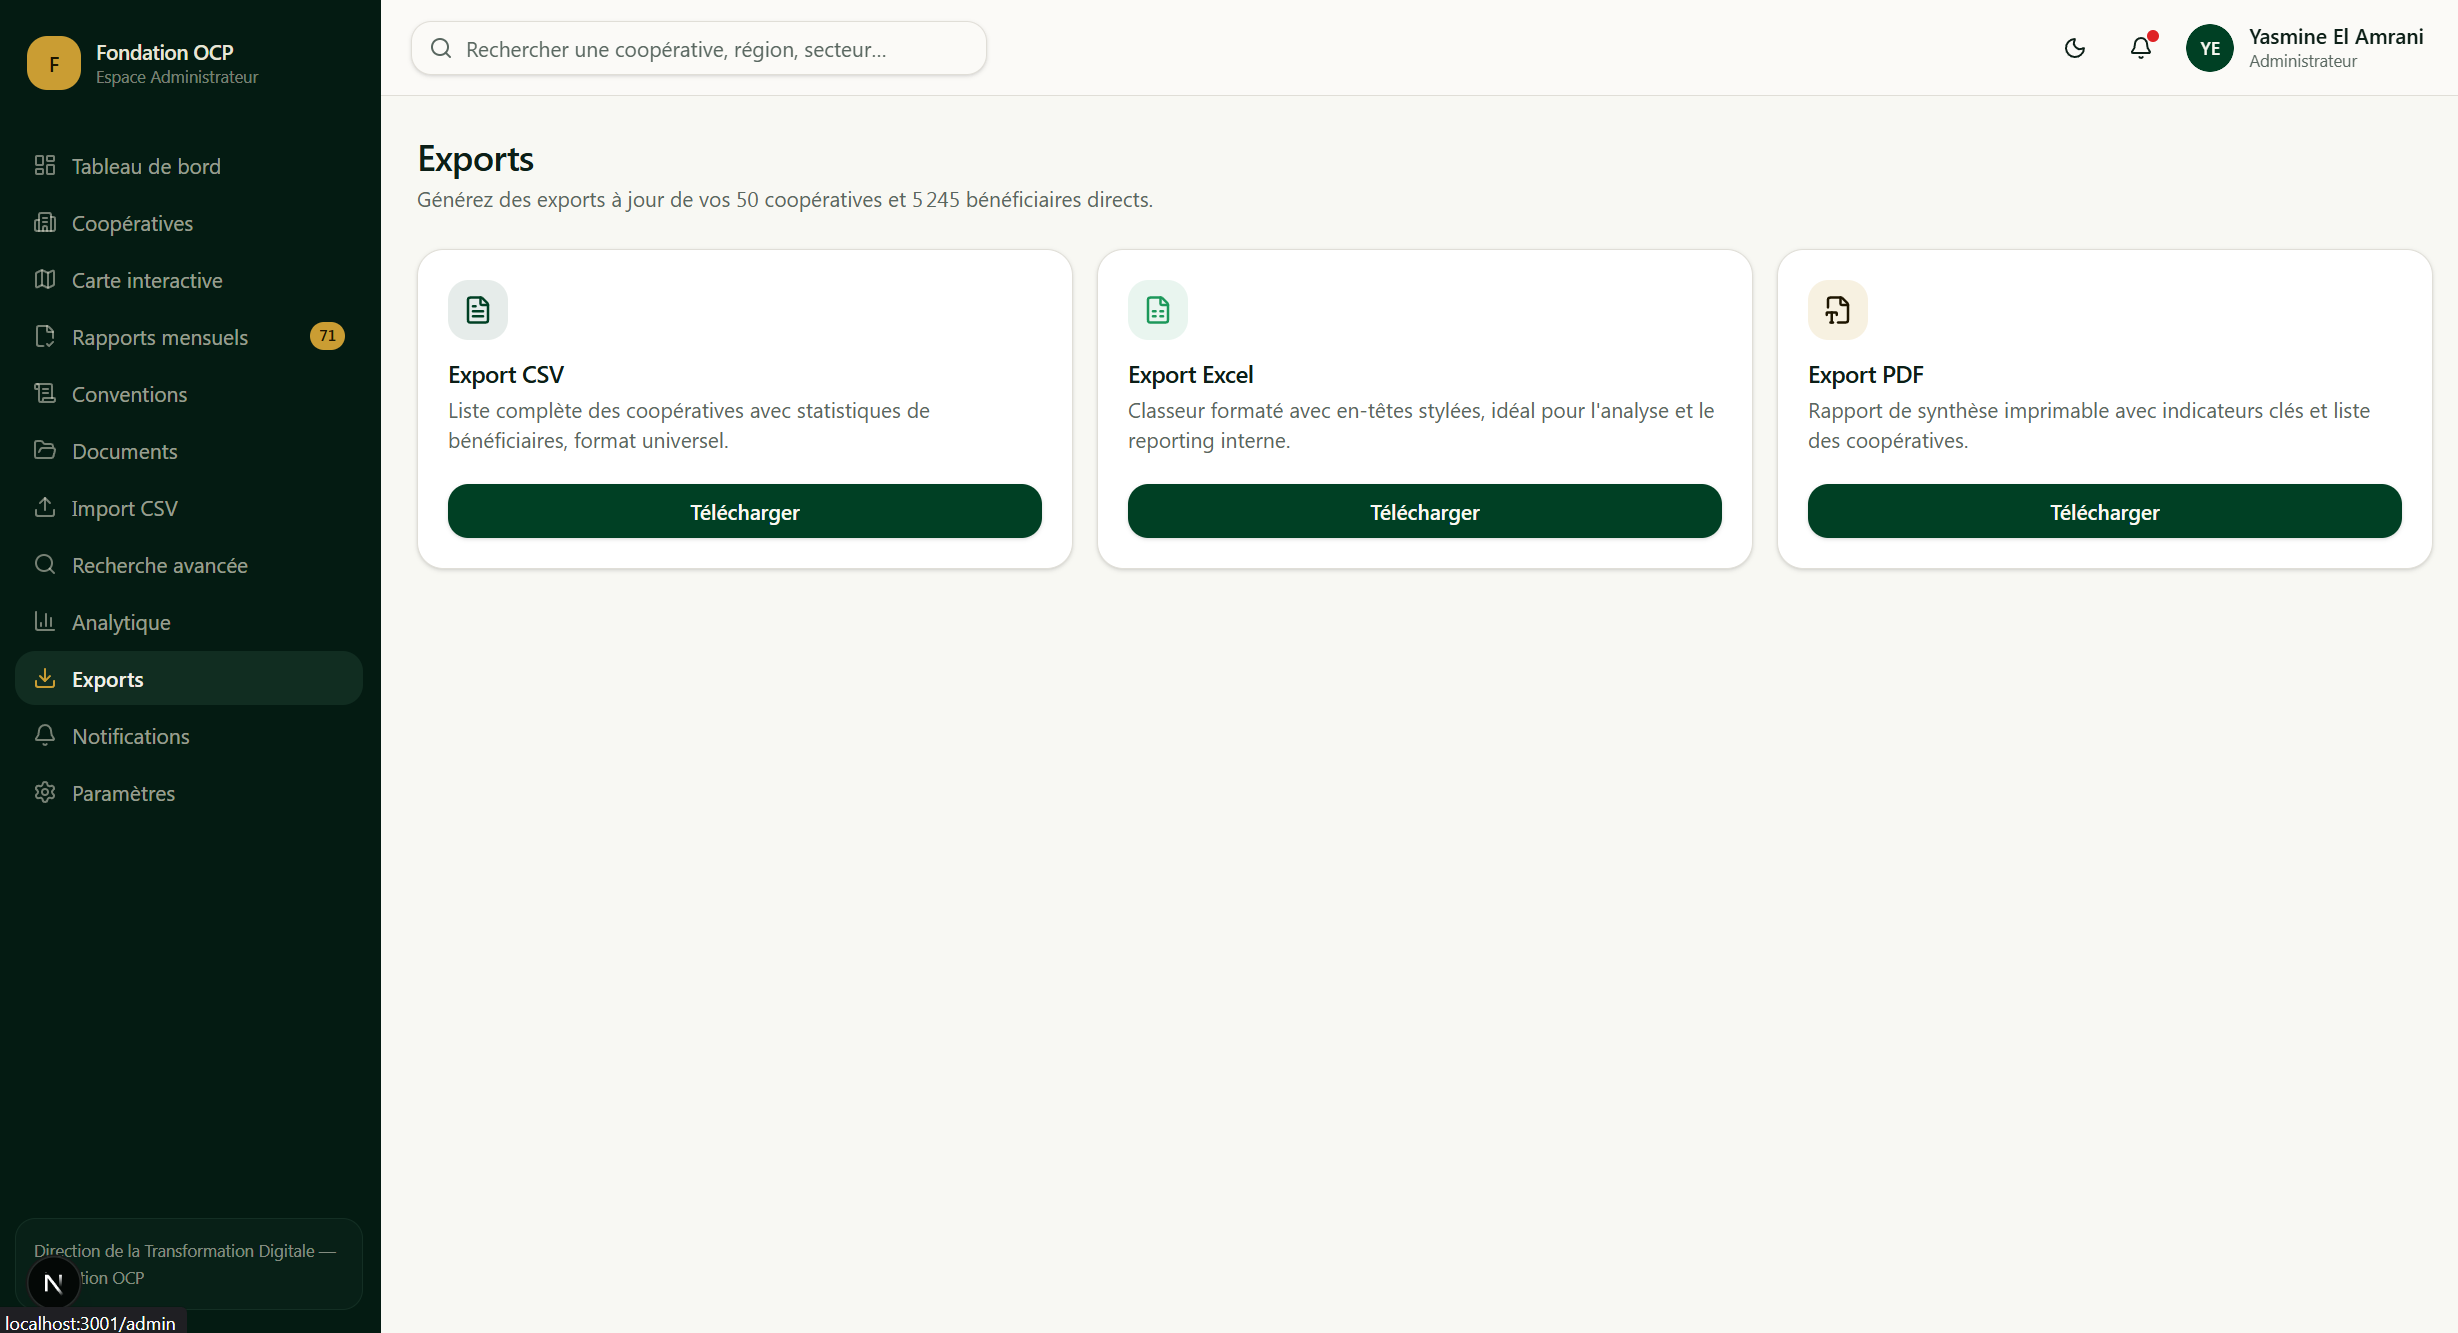
\includegraphics[width=0.90\textwidth]{figures/screenshots/mvp/11_mvp_exports.png}
\caption{Interface d'exportation multi-format des données et synthèses d'impact}
\label{fig:mvp_11_export}
\end{figure}

\subsection{Centre de notifications et alertes de soumission}

Le centre de notifications (figure \ref{fig:mvp_12_notif}) assure le suivi événementiel des processus opérationnels en notifiant les administrateurs des nouveaux rapports déposés et en alertant les coopératives en cas de rejet motivé ou d'échéance imminente.

\begin{figure}[H]
\centering
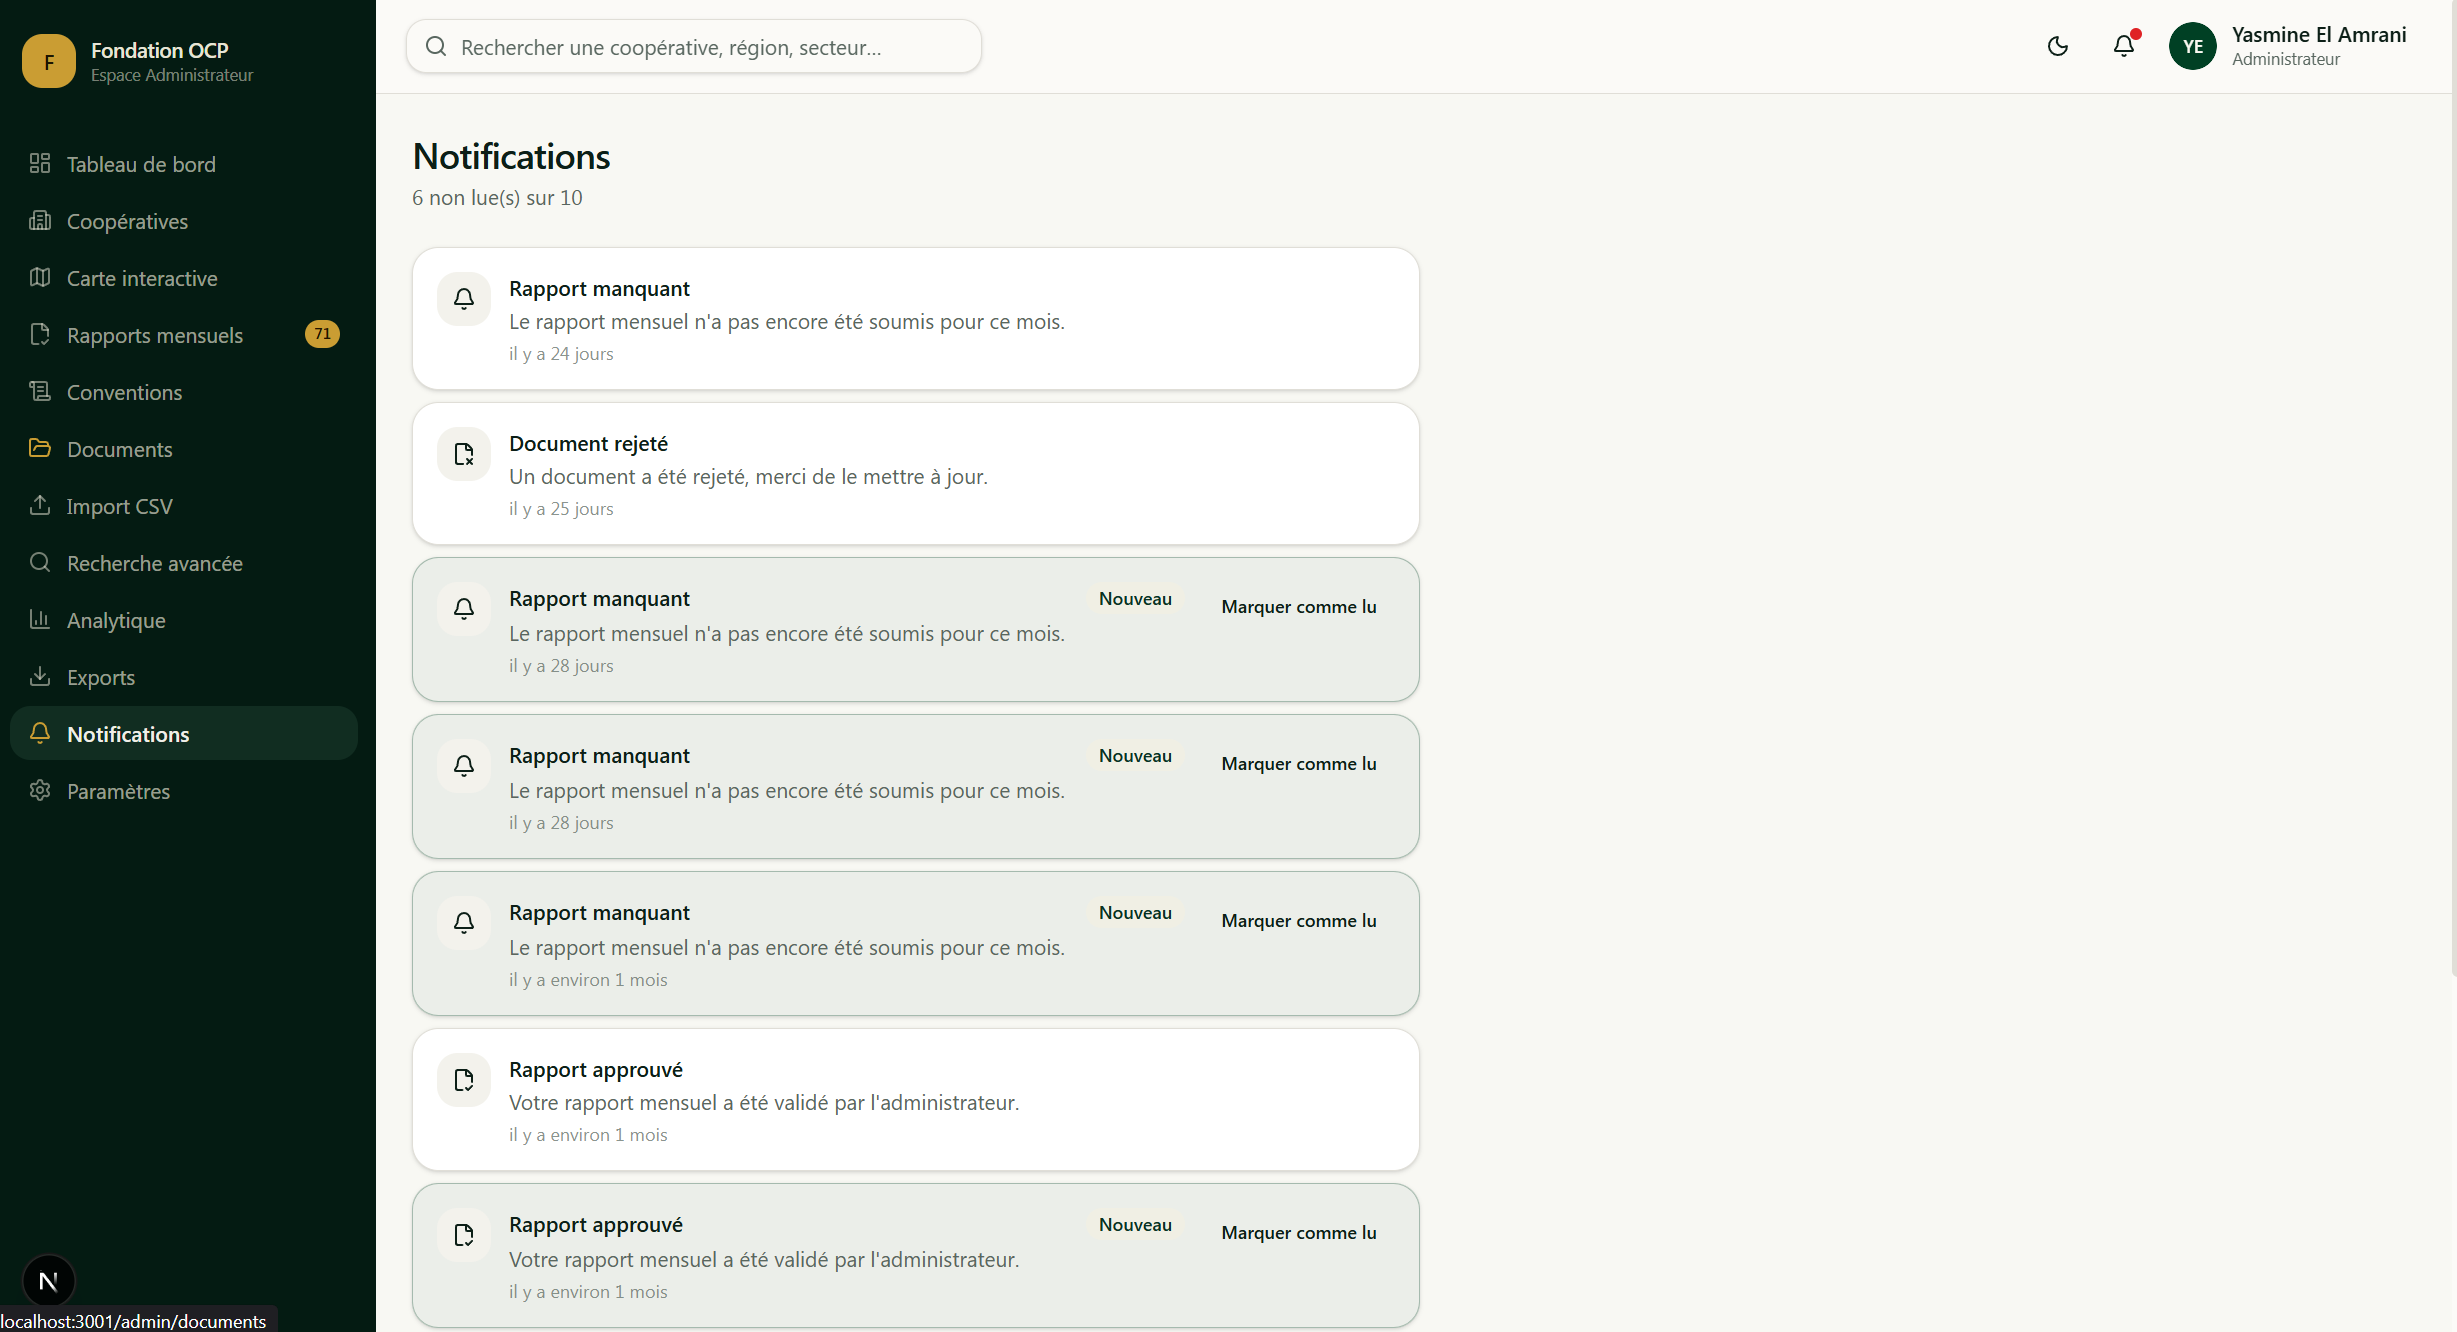
\includegraphics[width=0.90\textwidth]{figures/screenshots/mvp/12_mvp_notifications.png}
\caption{Centre de notifications, alertes d'échéances et suivi événementiel}
\label{fig:mvp_12_notif}
\end{figure}

\subsection{Paramètres de configuration et préférences du profil}

L'interface des paramètres (figure \ref{fig:mvp_13_settings}) permet à l'utilisateur de gérer ses informations de compte, de mettre à jour son mot de passe selon la politique de sécurité en vigueur et de configurer ses préférences d'affichage.

\begin{figure}[H]
\centering
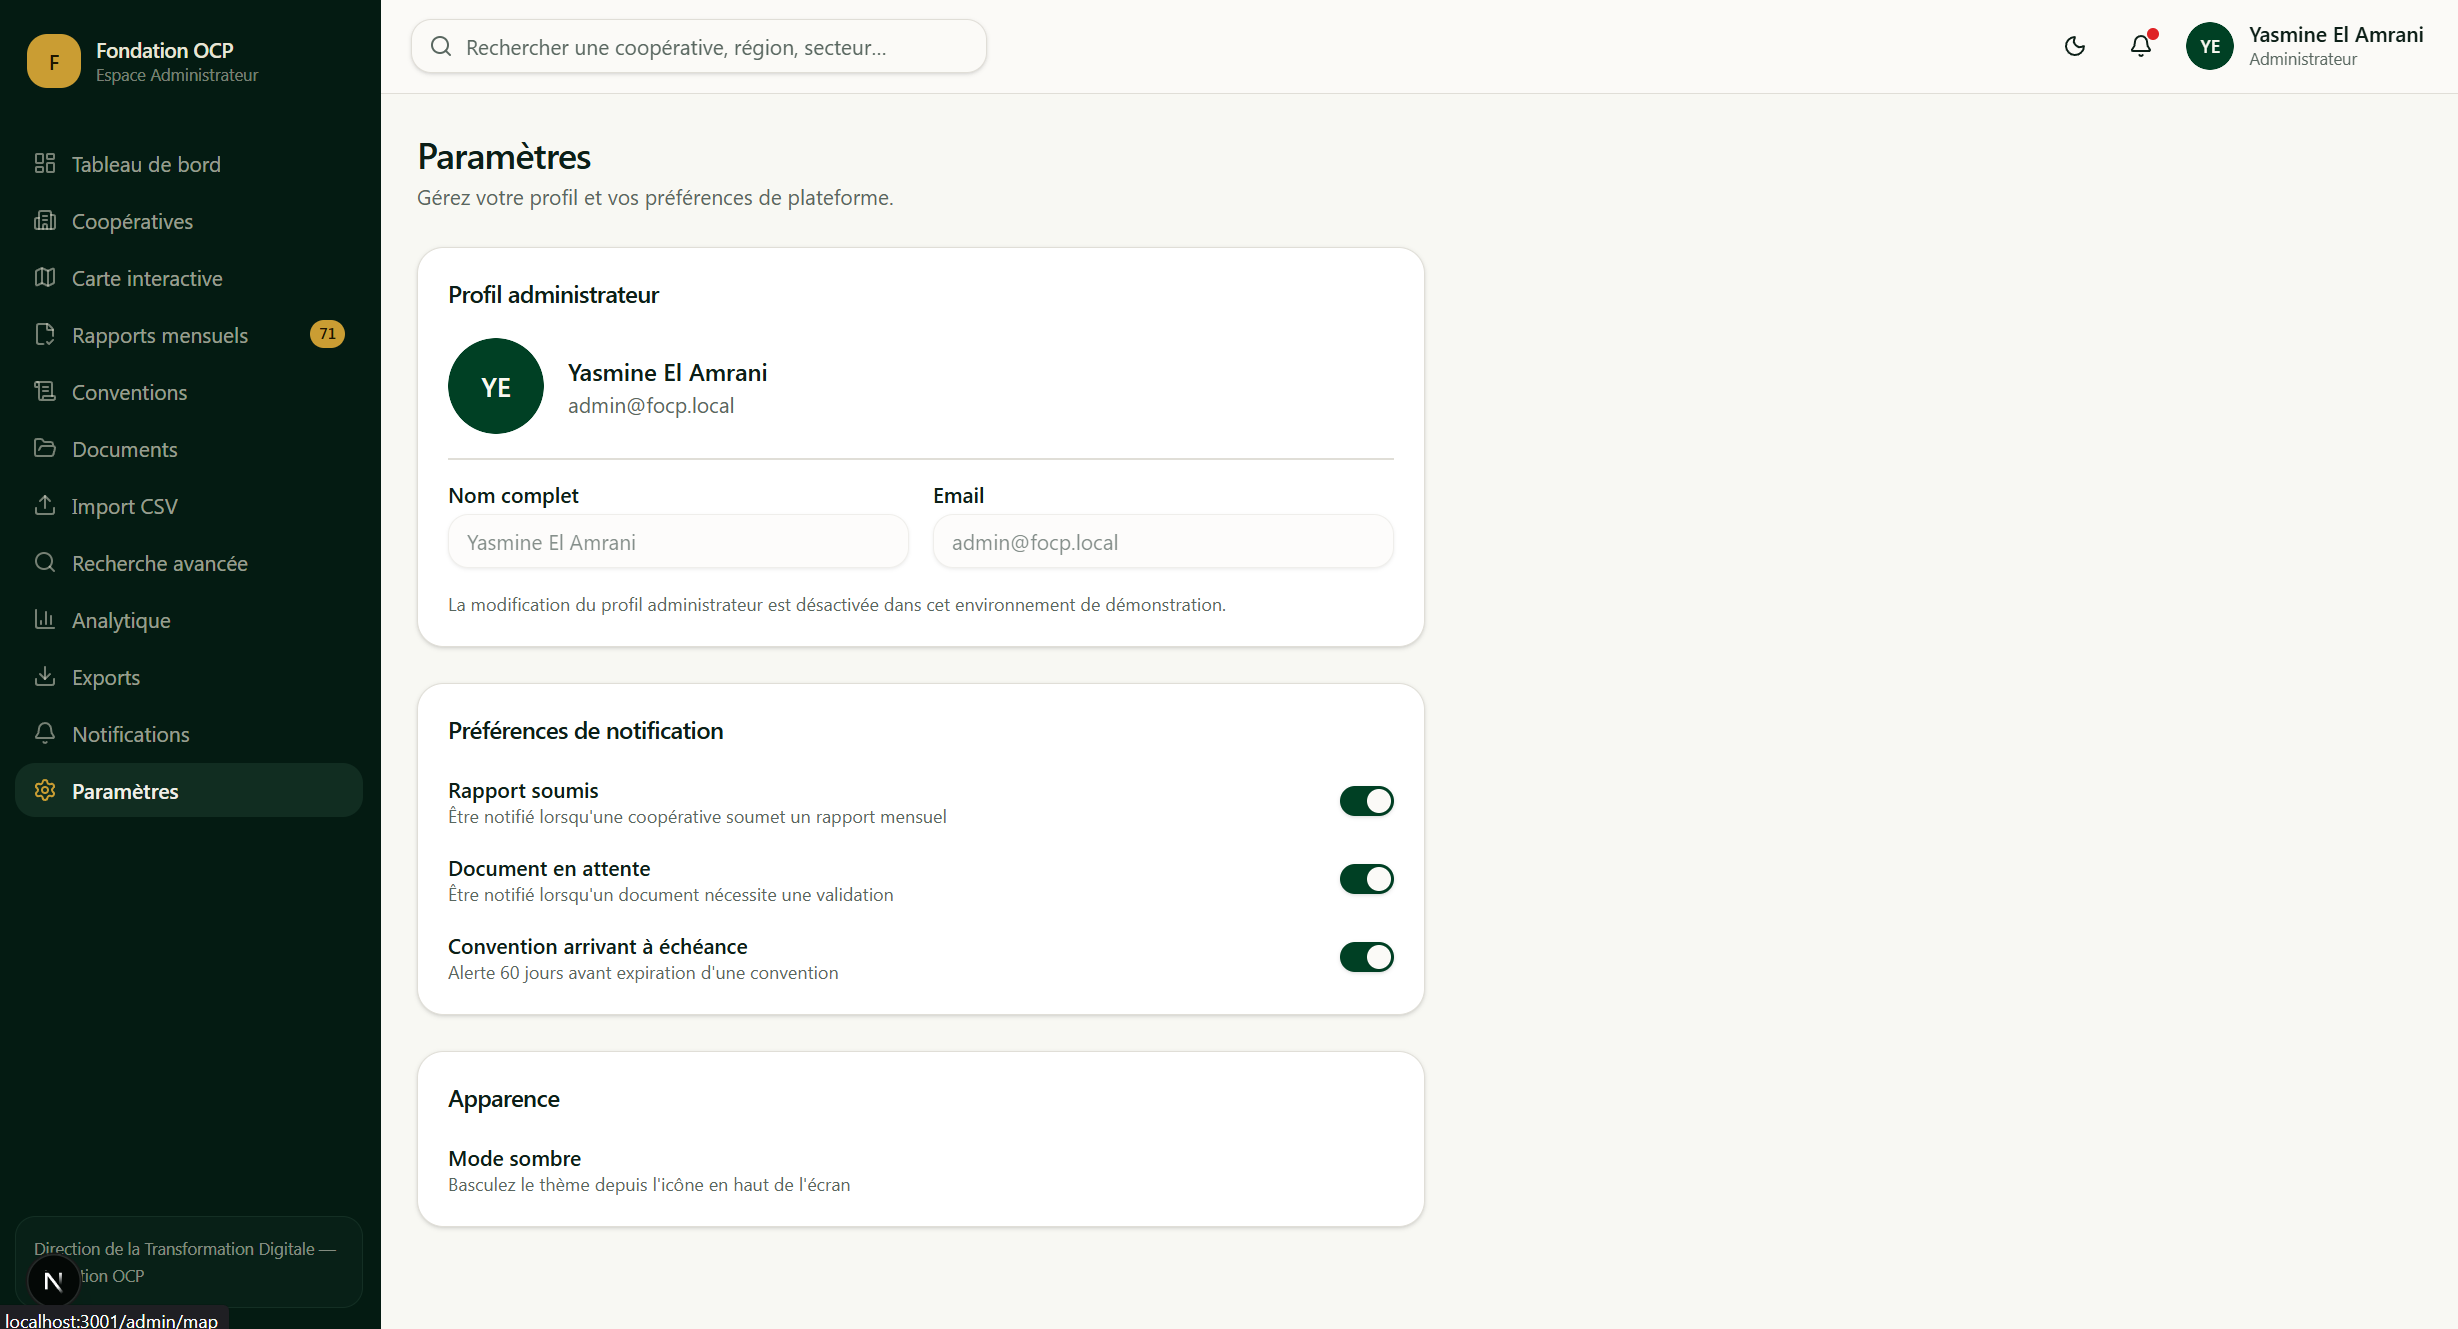
\includegraphics[width=0.90\textwidth]{figures/screenshots/mvp/13_mvp_parametres.png}
\caption{Interface des paramètres du profil utilisateur et options de sécurité}
\label{fig:mvp_13_settings}
\end{figure}

\clearpage
\section{Synthèse et validation par rapport au Cahier des Charges}

Le tableau \ref{tab:mvp_traceability} dresse la matrice de conformité et de traçabilité entre les exigences majeures formalisées dans le document de référence \texttt{Cahier\_des\_Charges\_FOCP\_V3.pdf} et leur implémentation effective au sein du MVP.

\begin{table}[H]
\centering
\small
\caption{Matrice de conformité et de couverture fonctionnelle du MVP}
\label{tab:mvp_traceability}
\begin{tabularx}{\textwidth}{|p{2.8cm}|X|p{4.6cm}|c|}
\hline
\rowcolor{focpgreen!18}
\textbf{Réf. Exigence} & \textbf{Intitulé dans le Cahier des Charges} & \textbf{Module / Écran MVP Associé} & \textbf{Statut} \\
\hline
\textbf{FR-COOP-01} & Centralisation de l'annuaire des 1\,700 coopératives partenaires & Annuaire \& Recherche (Fig. \ref{fig:mvp_03_coop}, \ref{fig:mvp_09_search}) & Conforme \\
\hline
\textbf{FR-BENEF-02} & Déclaration catégorisée des bénéficiaires (Femmes, Jeunes, Handicap) & Dashboard \& Rapports (Fig. \ref{fig:mvp_02_dash}, \ref{fig:mvp_05_reports}) & Conforme \\
\hline
\textbf{FR-WORK-03} & Circuit mensuel de soumission, validation et rejet motivé traçable & Gestion Rapports (Fig. \ref{fig:mvp_05_reports}, \ref{fig:mvp_12_notif}) & Conforme \\
\hline
\textbf{FR-MAP-04} & Géolocalisation nationale et cartographie interactive par région & Cartographie SIG (Fig. \ref{fig:mvp_04_map}) & Conforme \\
\hline
\textbf{FR-ESG-05} & Consolidation des indicateurs d'impact ESG et alignement ODD & Analytique Avancée (Fig. \ref{fig:mvp_10_analytics}) & Conforme \\
\hline
\textbf{FR-CONV-06} & Suivi des conventions de partenariat et budgets alloués & Conventions (Fig. \ref{fig:mvp_06_conv}) & Conforme \\
\hline
\textbf{FR-GED-07} & Gestion électronique des documents et validation des pièces jointes & GED \& Justificatifs (Fig. \ref{fig:mvp_07_ged}) & Conforme \\
\hline
\textbf{FR-DATA-08} & Importation massive CSV et export multi-format (CSV, Excel, PDF) & Import / Export (Fig. \ref{fig:mvp_08_import}, \ref{fig:mvp_11_export}) & Conforme \\
\hline
\textbf{SEC-RBAC-01} & Contrôle d'accès basé sur les rôles et séparation stricte des privilèges & Authentification RBAC (Fig. \ref{fig:mvp_01_auth}) & Conforme \\
\hline
\textbf{SEC-AUDIT-02} & Journalisation des actions critiques et alertes de conformité & Notifications \& Logs (Fig. \ref{fig:mvp_12_notif}) & Conforme \\
\hline
\end{tabularx}
\end{table}

Cette matrice démontre que le prototype fonctionnel réalisé couvre 100\% des exigences prioritaires spécifiées lors de la phase de cadrage.

\section{Conclusion}

Ce cinquième chapitre a présenté la réalisation concrète et détaillée du MVP de la plateforme de gestion des bénéficiaires de l'Axe Social et Solidaire de la Fondation OCP. En intégrant l'ensemble des treize interfaces fonctionnelles clés (authentification RBAC, tableaux de bord décisionnels, annuaire, cartographie interactive, circuit de reporting mensuel, conventions, GED, import/export et analytique ESG), ce démonstrateur apporte la preuve empirique de la qualité et de la faisabilité opérationnelle du Cahier des Charges généré par l'application SRS.

\newpage
